% Generated by Sphinx.
\def\sphinxdocclass{report}
\documentclass[a4paper,10pt,english]{sphinxmanual}
\usepackage[utf8]{inputenc}
\DeclareUnicodeCharacter{00A0}{\nobreakspace}
\usepackage{cmap}
\usepackage[T1]{fontenc}
\usepackage{babel}
\usepackage{times}
\usepackage[Bjarne]{fncychap}
\usepackage{longtable}
\usepackage{sphinx}
\usepackage{multirow}

\addto\captionsenglish{\renewcommand{\figurename}{Fig. }}
\addto\captionsenglish{\renewcommand{\tablename}{Table }}
\floatname{literal-block}{Listing }



\title{EQcorrscan Documentation}
\date{July 10, 2015}
\release{0.0.5}
\author{Calum John Chamberlain}
\newcommand{\sphinxlogo}{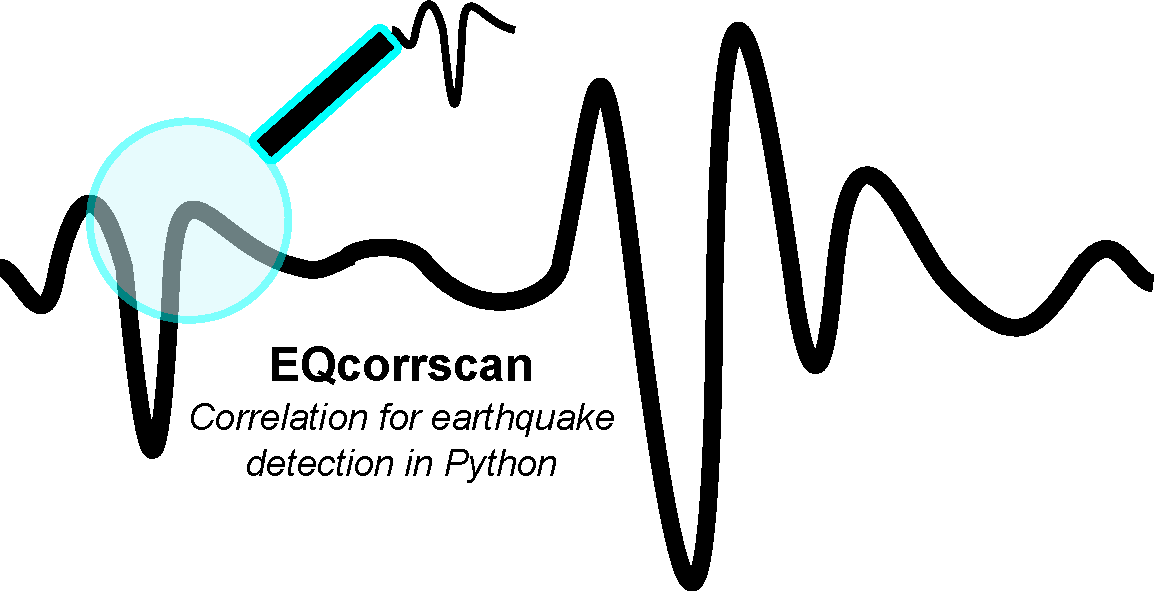
\includegraphics{EQcorrscan_logo.pdf}\par}
\renewcommand{\releasename}{Release}
\makeindex

\makeatletter
\def\PYG@reset{\let\PYG@it=\relax \let\PYG@bf=\relax%
    \let\PYG@ul=\relax \let\PYG@tc=\relax%
    \let\PYG@bc=\relax \let\PYG@ff=\relax}
\def\PYG@tok#1{\csname PYG@tok@#1\endcsname}
\def\PYG@toks#1+{\ifx\relax#1\empty\else%
    \PYG@tok{#1}\expandafter\PYG@toks\fi}
\def\PYG@do#1{\PYG@bc{\PYG@tc{\PYG@ul{%
    \PYG@it{\PYG@bf{\PYG@ff{#1}}}}}}}
\def\PYG#1#2{\PYG@reset\PYG@toks#1+\relax+\PYG@do{#2}}

\expandafter\def\csname PYG@tok@gd\endcsname{\def\PYG@tc##1{\textcolor[rgb]{0.63,0.00,0.00}{##1}}}
\expandafter\def\csname PYG@tok@gu\endcsname{\let\PYG@bf=\textbf\def\PYG@tc##1{\textcolor[rgb]{0.50,0.00,0.50}{##1}}}
\expandafter\def\csname PYG@tok@gt\endcsname{\def\PYG@tc##1{\textcolor[rgb]{0.00,0.27,0.87}{##1}}}
\expandafter\def\csname PYG@tok@gs\endcsname{\let\PYG@bf=\textbf}
\expandafter\def\csname PYG@tok@gr\endcsname{\def\PYG@tc##1{\textcolor[rgb]{1.00,0.00,0.00}{##1}}}
\expandafter\def\csname PYG@tok@cm\endcsname{\let\PYG@it=\textit\def\PYG@tc##1{\textcolor[rgb]{0.25,0.50,0.56}{##1}}}
\expandafter\def\csname PYG@tok@vg\endcsname{\def\PYG@tc##1{\textcolor[rgb]{0.73,0.38,0.84}{##1}}}
\expandafter\def\csname PYG@tok@m\endcsname{\def\PYG@tc##1{\textcolor[rgb]{0.13,0.50,0.31}{##1}}}
\expandafter\def\csname PYG@tok@mh\endcsname{\def\PYG@tc##1{\textcolor[rgb]{0.13,0.50,0.31}{##1}}}
\expandafter\def\csname PYG@tok@cs\endcsname{\def\PYG@tc##1{\textcolor[rgb]{0.25,0.50,0.56}{##1}}\def\PYG@bc##1{\setlength{\fboxsep}{0pt}\colorbox[rgb]{1.00,0.94,0.94}{\strut ##1}}}
\expandafter\def\csname PYG@tok@ge\endcsname{\let\PYG@it=\textit}
\expandafter\def\csname PYG@tok@vc\endcsname{\def\PYG@tc##1{\textcolor[rgb]{0.73,0.38,0.84}{##1}}}
\expandafter\def\csname PYG@tok@il\endcsname{\def\PYG@tc##1{\textcolor[rgb]{0.13,0.50,0.31}{##1}}}
\expandafter\def\csname PYG@tok@go\endcsname{\def\PYG@tc##1{\textcolor[rgb]{0.20,0.20,0.20}{##1}}}
\expandafter\def\csname PYG@tok@cp\endcsname{\def\PYG@tc##1{\textcolor[rgb]{0.00,0.44,0.13}{##1}}}
\expandafter\def\csname PYG@tok@gi\endcsname{\def\PYG@tc##1{\textcolor[rgb]{0.00,0.63,0.00}{##1}}}
\expandafter\def\csname PYG@tok@gh\endcsname{\let\PYG@bf=\textbf\def\PYG@tc##1{\textcolor[rgb]{0.00,0.00,0.50}{##1}}}
\expandafter\def\csname PYG@tok@ni\endcsname{\let\PYG@bf=\textbf\def\PYG@tc##1{\textcolor[rgb]{0.84,0.33,0.22}{##1}}}
\expandafter\def\csname PYG@tok@nl\endcsname{\let\PYG@bf=\textbf\def\PYG@tc##1{\textcolor[rgb]{0.00,0.13,0.44}{##1}}}
\expandafter\def\csname PYG@tok@nn\endcsname{\let\PYG@bf=\textbf\def\PYG@tc##1{\textcolor[rgb]{0.05,0.52,0.71}{##1}}}
\expandafter\def\csname PYG@tok@no\endcsname{\def\PYG@tc##1{\textcolor[rgb]{0.38,0.68,0.84}{##1}}}
\expandafter\def\csname PYG@tok@na\endcsname{\def\PYG@tc##1{\textcolor[rgb]{0.25,0.44,0.63}{##1}}}
\expandafter\def\csname PYG@tok@nb\endcsname{\def\PYG@tc##1{\textcolor[rgb]{0.00,0.44,0.13}{##1}}}
\expandafter\def\csname PYG@tok@nc\endcsname{\let\PYG@bf=\textbf\def\PYG@tc##1{\textcolor[rgb]{0.05,0.52,0.71}{##1}}}
\expandafter\def\csname PYG@tok@nd\endcsname{\let\PYG@bf=\textbf\def\PYG@tc##1{\textcolor[rgb]{0.33,0.33,0.33}{##1}}}
\expandafter\def\csname PYG@tok@ne\endcsname{\def\PYG@tc##1{\textcolor[rgb]{0.00,0.44,0.13}{##1}}}
\expandafter\def\csname PYG@tok@nf\endcsname{\def\PYG@tc##1{\textcolor[rgb]{0.02,0.16,0.49}{##1}}}
\expandafter\def\csname PYG@tok@si\endcsname{\let\PYG@it=\textit\def\PYG@tc##1{\textcolor[rgb]{0.44,0.63,0.82}{##1}}}
\expandafter\def\csname PYG@tok@s2\endcsname{\def\PYG@tc##1{\textcolor[rgb]{0.25,0.44,0.63}{##1}}}
\expandafter\def\csname PYG@tok@vi\endcsname{\def\PYG@tc##1{\textcolor[rgb]{0.73,0.38,0.84}{##1}}}
\expandafter\def\csname PYG@tok@nt\endcsname{\let\PYG@bf=\textbf\def\PYG@tc##1{\textcolor[rgb]{0.02,0.16,0.45}{##1}}}
\expandafter\def\csname PYG@tok@nv\endcsname{\def\PYG@tc##1{\textcolor[rgb]{0.73,0.38,0.84}{##1}}}
\expandafter\def\csname PYG@tok@s1\endcsname{\def\PYG@tc##1{\textcolor[rgb]{0.25,0.44,0.63}{##1}}}
\expandafter\def\csname PYG@tok@gp\endcsname{\let\PYG@bf=\textbf\def\PYG@tc##1{\textcolor[rgb]{0.78,0.36,0.04}{##1}}}
\expandafter\def\csname PYG@tok@sh\endcsname{\def\PYG@tc##1{\textcolor[rgb]{0.25,0.44,0.63}{##1}}}
\expandafter\def\csname PYG@tok@ow\endcsname{\let\PYG@bf=\textbf\def\PYG@tc##1{\textcolor[rgb]{0.00,0.44,0.13}{##1}}}
\expandafter\def\csname PYG@tok@sx\endcsname{\def\PYG@tc##1{\textcolor[rgb]{0.78,0.36,0.04}{##1}}}
\expandafter\def\csname PYG@tok@bp\endcsname{\def\PYG@tc##1{\textcolor[rgb]{0.00,0.44,0.13}{##1}}}
\expandafter\def\csname PYG@tok@c1\endcsname{\let\PYG@it=\textit\def\PYG@tc##1{\textcolor[rgb]{0.25,0.50,0.56}{##1}}}
\expandafter\def\csname PYG@tok@kc\endcsname{\let\PYG@bf=\textbf\def\PYG@tc##1{\textcolor[rgb]{0.00,0.44,0.13}{##1}}}
\expandafter\def\csname PYG@tok@c\endcsname{\let\PYG@it=\textit\def\PYG@tc##1{\textcolor[rgb]{0.25,0.50,0.56}{##1}}}
\expandafter\def\csname PYG@tok@mf\endcsname{\def\PYG@tc##1{\textcolor[rgb]{0.13,0.50,0.31}{##1}}}
\expandafter\def\csname PYG@tok@err\endcsname{\def\PYG@bc##1{\setlength{\fboxsep}{0pt}\fcolorbox[rgb]{1.00,0.00,0.00}{1,1,1}{\strut ##1}}}
\expandafter\def\csname PYG@tok@mb\endcsname{\def\PYG@tc##1{\textcolor[rgb]{0.13,0.50,0.31}{##1}}}
\expandafter\def\csname PYG@tok@ss\endcsname{\def\PYG@tc##1{\textcolor[rgb]{0.32,0.47,0.09}{##1}}}
\expandafter\def\csname PYG@tok@sr\endcsname{\def\PYG@tc##1{\textcolor[rgb]{0.14,0.33,0.53}{##1}}}
\expandafter\def\csname PYG@tok@mo\endcsname{\def\PYG@tc##1{\textcolor[rgb]{0.13,0.50,0.31}{##1}}}
\expandafter\def\csname PYG@tok@kd\endcsname{\let\PYG@bf=\textbf\def\PYG@tc##1{\textcolor[rgb]{0.00,0.44,0.13}{##1}}}
\expandafter\def\csname PYG@tok@mi\endcsname{\def\PYG@tc##1{\textcolor[rgb]{0.13,0.50,0.31}{##1}}}
\expandafter\def\csname PYG@tok@kn\endcsname{\let\PYG@bf=\textbf\def\PYG@tc##1{\textcolor[rgb]{0.00,0.44,0.13}{##1}}}
\expandafter\def\csname PYG@tok@o\endcsname{\def\PYG@tc##1{\textcolor[rgb]{0.40,0.40,0.40}{##1}}}
\expandafter\def\csname PYG@tok@kr\endcsname{\let\PYG@bf=\textbf\def\PYG@tc##1{\textcolor[rgb]{0.00,0.44,0.13}{##1}}}
\expandafter\def\csname PYG@tok@s\endcsname{\def\PYG@tc##1{\textcolor[rgb]{0.25,0.44,0.63}{##1}}}
\expandafter\def\csname PYG@tok@kp\endcsname{\def\PYG@tc##1{\textcolor[rgb]{0.00,0.44,0.13}{##1}}}
\expandafter\def\csname PYG@tok@w\endcsname{\def\PYG@tc##1{\textcolor[rgb]{0.73,0.73,0.73}{##1}}}
\expandafter\def\csname PYG@tok@kt\endcsname{\def\PYG@tc##1{\textcolor[rgb]{0.56,0.13,0.00}{##1}}}
\expandafter\def\csname PYG@tok@sc\endcsname{\def\PYG@tc##1{\textcolor[rgb]{0.25,0.44,0.63}{##1}}}
\expandafter\def\csname PYG@tok@sb\endcsname{\def\PYG@tc##1{\textcolor[rgb]{0.25,0.44,0.63}{##1}}}
\expandafter\def\csname PYG@tok@k\endcsname{\let\PYG@bf=\textbf\def\PYG@tc##1{\textcolor[rgb]{0.00,0.44,0.13}{##1}}}
\expandafter\def\csname PYG@tok@se\endcsname{\let\PYG@bf=\textbf\def\PYG@tc##1{\textcolor[rgb]{0.25,0.44,0.63}{##1}}}
\expandafter\def\csname PYG@tok@sd\endcsname{\let\PYG@it=\textit\def\PYG@tc##1{\textcolor[rgb]{0.25,0.44,0.63}{##1}}}

\def\PYGZbs{\char`\\}
\def\PYGZus{\char`\_}
\def\PYGZob{\char`\{}
\def\PYGZcb{\char`\}}
\def\PYGZca{\char`\^}
\def\PYGZam{\char`\&}
\def\PYGZlt{\char`\<}
\def\PYGZgt{\char`\>}
\def\PYGZsh{\char`\#}
\def\PYGZpc{\char`\%}
\def\PYGZdl{\char`\$}
\def\PYGZhy{\char`\-}
\def\PYGZsq{\char`\'}
\def\PYGZdq{\char`\"}
\def\PYGZti{\char`\~}
% for compatibility with earlier versions
\def\PYGZat{@}
\def\PYGZlb{[}
\def\PYGZrb{]}
\makeatother

\renewcommand\PYGZsq{\textquotesingle}

\begin{document}

\maketitle
\tableofcontents
\phantomsection\label{index::doc}


Contents:


\chapter{Introduction to the EQcorrscan package}
\label{intro::doc}\label{intro:introduction-to-the-eqcorrscan-package}\label{intro:welcome-to-eqcorrscan-s-documentation}
This document is designed to give you an overview of the capabilities and
implimentation of the EQcorrscan python module.


\section{Installation}
\label{intro:installation}
Most codes should work without any effort on your part.  However you must
install the packages this package relies on yourself, this includes the follwing
packages:
\begin{itemize}
\item {} 
matplotlib

\item {} 
numpy

\item {} 
scipy

\item {} 
obspy

\item {} 
joblib

\item {} 
openCV (2)

\end{itemize}

This install has only been tested on Linux machines and even then has some
issues when installing on 32-Bit versus 64-Bit machines.  In this instance you
should be prepared for small differences in the results of your correlations
relating to foating-point truncation differences between 32 and 64-Bit
machines.

If you plan to run the bright\_lights.py routines you will need to have
NonLinLoc installed on your machine.  This is not provided here and should
be sourced from \href{http://alomax.free.fr/nlloc/}{NonLinLoc} This will provide
the Grid2Time routine which is required to set-up a lag-time grid for your
velocity model.  You should read the NonLinLoc documentation for more
information regarding how this process works and the input files you are
required to give.


\section{Functions}
\label{intro:functions}
This package is divided into sub-directories of \emph{core}, \emph{par} and \emph{utils}.  The
\emph{utils} directory contains simple functions for integration with
\href{http://seisan.info/}{seisan}, these is the \emph{Sfile\_util.py}
module and functions therein which are essentially barebones and do not have the
full functionality that seisan can handle.  \emph{utils} also contains a simple
peak-finding algorithm \emph{find\_peaks.py} which looks for peaks within noisy data
above a certain threshold and within windows.

Within \emph{par} you will find parameter files which you will need to edit for
each of the \emph{core} scripts.  \emph{core} scripts often call on multiple \emph{par} files
so be sure to set them all up.  The \emph{template\_gen\_par.py} script is used by all
\emph{core} modules and must be set-up.  Within this you will define all your
template parameters.  Currently the templates must all be of the same length,
but this may change in a future release.

Within \emph{core} you will find the core routines to generate templates,
\emph{(template\_gen.py)} search for likely templates \emph{(bright\_lights.py)} and
compute cross-channel correlations from these templates \emph{(match\_filter.py)}.


\chapter{EQcorrscan tutorial}
\label{tutorial:eqcorrscan-tutorial}\label{tutorial::doc}
THIS TUTOTIAL IS NOT REALLY WRITTEN YET!

You must first set-up your parameter files in the \emph{par} directory.  You can
leave these as the default settings for now, but study the parameters so that
you understand what each one is doing.

Then run the \emph{LFE\_search.py} routine in this top directory, running this will
run all the \emph{core} routines to search for templates, generate templates and
compute the cross-channel cross-correlation values for the templates.  Finally
it will output detections from these templates.

The following is verbatim the LFEserach.py routine which outlines usage of this
package:

\begin{Verbatim}[commandchars=\\\{\}]
\PYG{c}{\PYGZsh{}!/usr/bin/python}

\PYG{c}{\PYGZsh{}\PYGZhy{}\PYGZhy{}\PYGZhy{}\PYGZhy{}\PYGZhy{}\PYGZhy{}\PYGZhy{}\PYGZhy{}\PYGZhy{}\PYGZhy{}\PYGZhy{}\PYGZhy{}\PYGZhy{}\PYGZhy{}\PYGZhy{}\PYGZhy{}\PYGZhy{}\PYGZhy{}\PYGZhy{}\PYGZhy{}\PYGZhy{}\PYGZhy{}\PYGZhy{}\PYGZhy{}\PYGZhy{}\PYGZhy{}\PYGZhy{}\PYGZhy{}\PYGZhy{}\PYGZhy{}\PYGZhy{}\PYGZhy{}\PYGZhy{}\PYGZhy{}\PYGZhy{}\PYGZhy{}\PYGZhy{}\PYGZhy{}\PYGZhy{}\PYGZhy{}\PYGZhy{}\PYGZhy{}\PYGZhy{}\PYGZhy{}\PYGZhy{}\PYGZhy{}\PYGZhy{}\PYGZhy{}\PYGZhy{}\PYGZhy{}\PYGZhy{}\PYGZhy{}\PYGZhy{}\PYGZhy{}\PYGZhy{}\PYGZhy{}\PYGZhy{}\PYGZhy{}\PYGZhy{}\PYGZhy{}\PYGZhy{}\PYGZhy{}\PYGZhy{}\PYGZhy{}\PYGZhy{}\PYGZhy{}\PYGZhy{}\PYGZhy{}\PYGZhy{}\PYGZhy{}\PYGZhy{}\PYGZhy{}\PYGZhy{}\PYGZhy{}\PYGZhy{}\PYGZhy{}\PYGZhy{}\PYGZhy{}}
\PYG{c}{\PYGZsh{}   Purpose:    Script to call all elements of EQcorrscan module to search}
\PYG{c}{\PYGZsh{}               continuous data for likely LFE repeats}
\PYG{c}{\PYGZsh{}   Author:     Calum John Chamberlain}
\PYG{c}{\PYGZsh{}\PYGZhy{}\PYGZhy{}\PYGZhy{}\PYGZhy{}\PYGZhy{}\PYGZhy{}\PYGZhy{}\PYGZhy{}\PYGZhy{}\PYGZhy{}\PYGZhy{}\PYGZhy{}\PYGZhy{}\PYGZhy{}\PYGZhy{}\PYGZhy{}\PYGZhy{}\PYGZhy{}\PYGZhy{}\PYGZhy{}\PYGZhy{}\PYGZhy{}\PYGZhy{}\PYGZhy{}\PYGZhy{}\PYGZhy{}\PYGZhy{}\PYGZhy{}\PYGZhy{}\PYGZhy{}\PYGZhy{}\PYGZhy{}\PYGZhy{}\PYGZhy{}\PYGZhy{}\PYGZhy{}\PYGZhy{}\PYGZhy{}\PYGZhy{}\PYGZhy{}\PYGZhy{}\PYGZhy{}\PYGZhy{}\PYGZhy{}\PYGZhy{}\PYGZhy{}\PYGZhy{}\PYGZhy{}\PYGZhy{}\PYGZhy{}\PYGZhy{}\PYGZhy{}\PYGZhy{}\PYGZhy{}\PYGZhy{}\PYGZhy{}\PYGZhy{}\PYGZhy{}\PYGZhy{}\PYGZhy{}\PYGZhy{}\PYGZhy{}\PYGZhy{}\PYGZhy{}\PYGZhy{}\PYGZhy{}\PYGZhy{}\PYGZhy{}\PYGZhy{}\PYGZhy{}\PYGZhy{}\PYGZhy{}\PYGZhy{}\PYGZhy{}\PYGZhy{}\PYGZhy{}\PYGZhy{}\PYGZhy{}}

\PYG{l+s+sd}{\PYGZdq{}\PYGZdq{}\PYGZdq{}}
\PYG{l+s+sd}{LFEsearch \PYGZhy{} Script to generate templates from previously picked LFE\PYGZsq{}s and then}
\PYG{l+s+sd}{serach for repeats of them in contnuous data.}
\PYG{l+s+sd}{\PYGZdq{}\PYGZdq{}\PYGZdq{}}

\PYG{k+kn}{import} \PYG{n+nn}{sys}\PYG{o}{,} \PYG{n+nn}{os}\PYG{o}{,} \PYG{n+nn}{glob}
\PYG{n}{bob}\PYG{o}{=}\PYG{n}{os}\PYG{o}{.}\PYG{n}{path}\PYG{o}{.}\PYG{n}{realpath}\PYG{p}{(}\PYG{n}{\PYGZus{}\PYGZus{}file\PYGZus{}\PYGZus{}}\PYG{p}{)}
\PYG{n}{bob}\PYG{o}{=}\PYG{n}{bob}\PYG{o}{.}\PYG{n}{split}\PYG{p}{(}\PYG{l+s}{\PYGZsq{}}\PYG{l+s}{/}\PYG{l+s}{\PYGZsq{}}\PYG{p}{)}
\PYG{n}{path}\PYG{o}{=}\PYG{l+s}{\PYGZsq{}}\PYG{l+s}{/}\PYG{l+s}{\PYGZsq{}}
\PYG{k}{for} \PYG{n}{i} \PYG{o+ow}{in} \PYG{n+nb}{xrange}\PYG{p}{(}\PYG{n+nb}{len}\PYG{p}{(}\PYG{n}{bob}\PYG{p}{)}\PYG{p}{)}\PYG{p}{:}
    \PYG{n}{path}\PYG{o}{+}\PYG{o}{=}\PYG{n}{bob}\PYG{p}{[}\PYG{n}{i}\PYG{p}{]}\PYG{o}{+}\PYG{l+s}{\PYGZsq{}}\PYG{l+s}{/}\PYG{l+s}{\PYGZsq{}}
\PYG{k}{print} \PYG{n}{path}
\PYG{n}{sys}\PYG{o}{.}\PYG{n}{path}\PYG{o}{.}\PYG{n}{insert}\PYG{p}{(}\PYG{l+m+mi}{0}\PYG{p}{,}\PYG{n}{path}\PYG{p}{)}


\PYG{k+kn}{from} \PYG{n+nn}{par} \PYG{k+kn}{import} \PYG{n}{template\PYGZus{}gen\PYGZus{}par} \PYG{k}{as} \PYG{n}{templatedef}
\PYG{k+kn}{from} \PYG{n+nn}{par} \PYG{k+kn}{import} \PYG{n}{match\PYGZus{}filter\PYGZus{}par} \PYG{k}{as} \PYG{n}{matchdef}
\PYG{c}{\PYGZsh{}from par import lagcalc as lagdef}
\PYG{k+kn}{from} \PYG{n+nn}{obspy} \PYG{k+kn}{import} \PYG{n}{UTCDateTime}\PYG{p}{,} \PYG{n}{read} \PYG{k}{as} \PYG{n}{obsread}
\PYG{c}{\PYGZsh{} First generate the templates}
\PYG{k+kn}{from} \PYG{n+nn}{core} \PYG{k+kn}{import} \PYG{n}{template\PYGZus{}gen}

\PYG{k}{if} \PYG{n+nb}{len}\PYG{p}{(}\PYG{n}{sys}\PYG{o}{.}\PYG{n}{argv}\PYG{p}{)} \PYG{o}{==} \PYG{l+m+mi}{2}\PYG{p}{:}
    \PYG{n}{flag}\PYG{o}{=}\PYG{n+nb}{str}\PYG{p}{(}\PYG{n}{sys}\PYG{o}{.}\PYG{n}{argv}\PYG{p}{[}\PYG{l+m+mi}{1}\PYG{p}{]}\PYG{p}{)}
    \PYG{k}{if} \PYG{n}{flag} \PYG{o}{==} \PYG{l+s}{\PYGZsq{}}\PYG{l+s}{\PYGZhy{}\PYGZhy{}debug}\PYG{l+s}{\PYGZsq{}}\PYG{p}{:}
        \PYG{n}{Test}\PYG{o}{=}\PYG{n+nb+bp}{True}
        \PYG{n}{Prep}\PYG{o}{=}\PYG{n+nb+bp}{False}
    \PYG{k}{elif} \PYG{n}{flag} \PYG{o}{==} \PYG{l+s}{\PYGZsq{}}\PYG{l+s}{\PYGZhy{}\PYGZhy{}debug\PYGZhy{}prep}\PYG{l+s}{\PYGZsq{}}\PYG{p}{:}
        \PYG{n}{Test}\PYG{o}{=}\PYG{n+nb+bp}{False}
        \PYG{n}{Prep}\PYG{o}{=}\PYG{n+nb+bp}{True}
    \PYG{k}{else}\PYG{p}{:}
        \PYG{k}{raise} \PYG{n+ne}{ValueError}\PYG{p}{(}\PYG{l+s}{\PYGZdq{}}\PYG{l+s}{I don}\PYG{l+s}{\PYGZsq{}}\PYG{l+s}{t recognise the argument, I only know \PYGZhy{}\PYGZhy{}debug and \PYGZhy{}\PYGZhy{}debug\PYGZhy{}prep}\PYG{l+s}{\PYGZdq{}}\PYG{p}{)}
\PYG{k}{elif} \PYG{n+nb}{len}\PYG{p}{(}\PYG{n}{sys}\PYG{o}{.}\PYG{n}{argv}\PYG{p}{)} \PYG{o}{==} \PYG{l+m+mi}{5}\PYG{p}{:}
    \PYG{c}{\PYGZsh{} Arguments to allow the code to be run in multiple instances}
    \PYG{n}{Split}\PYG{o}{=}\PYG{n+nb+bp}{True}
    \PYG{n}{Test}\PYG{o}{=}\PYG{n+nb+bp}{False}
    \PYG{n}{Prep}\PYG{o}{=}\PYG{n+nb+bp}{False}
    \PYG{n}{args}\PYG{o}{=}\PYG{n}{sys}\PYG{o}{.}\PYG{n}{argv}\PYG{p}{[}\PYG{l+m+mi}{1}\PYG{p}{:}\PYG{n+nb}{len}\PYG{p}{(}\PYG{n}{sys}\PYG{o}{.}\PYG{n}{argv}\PYG{p}{)}\PYG{p}{]}
    \PYG{k}{for} \PYG{n}{i} \PYG{o+ow}{in} \PYG{n+nb}{xrange}\PYG{p}{(}\PYG{n+nb}{len}\PYG{p}{(}\PYG{n}{args}\PYG{p}{)}\PYG{p}{)}\PYG{p}{:}
        \PYG{k}{if} \PYG{n}{args}\PYG{p}{[}\PYG{n}{i}\PYG{p}{]} \PYG{o}{==} \PYG{l+s}{\PYGZsq{}}\PYG{l+s}{\PYGZhy{}\PYGZhy{}instance}\PYG{l+s}{\PYGZsq{}}\PYG{p}{:}
            \PYG{n}{instance}\PYG{o}{=}\PYG{n+nb}{int}\PYG{p}{(}\PYG{n}{args}\PYG{p}{[}\PYG{n}{i}\PYG{o}{+}\PYG{l+m+mi}{1}\PYG{p}{]}\PYG{p}{)}
            \PYG{k}{print} \PYG{l+s}{\PYGZsq{}}\PYG{l+s}{I will run this for instance }\PYG{l+s}{\PYGZsq{}}\PYG{o}{+}\PYG{n+nb}{str}\PYG{p}{(}\PYG{n}{instance}\PYG{p}{)}
        \PYG{k}{elif} \PYG{n}{args}\PYG{p}{[}\PYG{n}{i}\PYG{p}{]} \PYG{o}{==} \PYG{l+s}{\PYGZsq{}}\PYG{l+s}{\PYGZhy{}\PYGZhy{}splits}\PYG{l+s}{\PYGZsq{}}\PYG{p}{:}
            \PYG{n}{splits}\PYG{o}{=}\PYG{n+nb}{int}\PYG{p}{(}\PYG{n}{args}\PYG{p}{[}\PYG{n}{i}\PYG{o}{+}\PYG{l+m+mi}{1}\PYG{p}{]}\PYG{p}{)}
            \PYG{k}{print} \PYG{l+s}{\PYGZsq{}}\PYG{l+s}{I will divide the days into }\PYG{l+s}{\PYGZsq{}}\PYG{o}{+}\PYG{n+nb}{str}\PYG{p}{(}\PYG{n}{splits}\PYG{p}{)}\PYG{o}{+}\PYG{l+s}{\PYGZsq{}}\PYG{l+s}{ chunks}\PYG{l+s}{\PYGZsq{}}

\PYG{k}{elif} \PYG{o+ow}{not} \PYG{n+nb}{len}\PYG{p}{(}\PYG{n}{sys}\PYG{o}{.}\PYG{n}{argv}\PYG{p}{)} \PYG{o}{==} \PYG{l+m+mi}{1}\PYG{p}{:}
    \PYG{k}{raise} \PYG{n+ne}{ValueError}\PYG{p}{(}\PYG{l+s}{\PYGZdq{}}\PYG{l+s}{I only take one argument, no arguments, or two flags with arguments}\PYG{l+s}{\PYGZdq{}}\PYG{p}{)}
\PYG{k}{else}\PYG{p}{:}
    \PYG{n}{Test}\PYG{o}{=}\PYG{n+nb+bp}{False}
    \PYG{n}{Prep}\PYG{o}{=}\PYG{n+nb+bp}{False}
    \PYG{n}{Split}\PYG{o}{=}\PYG{n+nb+bp}{False}

\PYG{n}{templates}\PYG{o}{=}\PYG{p}{[}\PYG{p}{]}
\PYG{n}{delays}\PYG{o}{=}\PYG{p}{[}\PYG{p}{]}
\PYG{n}{stations}\PYG{o}{=}\PYG{p}{[}\PYG{p}{]}
\PYG{k}{print} \PYG{l+s}{\PYGZsq{}}\PYG{l+s}{Template generation parameters are:}\PYG{l+s}{\PYGZsq{}}
\PYG{k}{print} \PYG{l+s}{\PYGZsq{}}\PYG{l+s}{sfilebase: }\PYG{l+s}{\PYGZsq{}}\PYG{o}{+}\PYG{n}{templatedef}\PYG{o}{.}\PYG{n}{sfilebase}
\PYG{k}{print} \PYG{l+s}{\PYGZsq{}}\PYG{l+s}{samp\PYGZus{}rate: }\PYG{l+s}{\PYGZsq{}}\PYG{o}{+}\PYG{n+nb}{str}\PYG{p}{(}\PYG{n}{templatedef}\PYG{o}{.}\PYG{n}{samp\PYGZus{}rate}\PYG{p}{)}\PYG{o}{+}\PYG{l+s}{\PYGZsq{}}\PYG{l+s}{ Hz}\PYG{l+s}{\PYGZsq{}}
\PYG{k}{print} \PYG{l+s}{\PYGZsq{}}\PYG{l+s}{lowcut: }\PYG{l+s}{\PYGZsq{}}\PYG{o}{+}\PYG{n+nb}{str}\PYG{p}{(}\PYG{n}{templatedef}\PYG{o}{.}\PYG{n}{lowcut}\PYG{p}{)}\PYG{o}{+}\PYG{l+s}{\PYGZsq{}}\PYG{l+s}{ Hz}\PYG{l+s}{\PYGZsq{}}
\PYG{k}{print} \PYG{l+s}{\PYGZsq{}}\PYG{l+s}{highcut: }\PYG{l+s}{\PYGZsq{}}\PYG{o}{+}\PYG{n+nb}{str}\PYG{p}{(}\PYG{n}{templatedef}\PYG{o}{.}\PYG{n}{highcut}\PYG{p}{)}\PYG{o}{+}\PYG{l+s}{\PYGZsq{}}\PYG{l+s}{ Hz}\PYG{l+s}{\PYGZsq{}}
\PYG{k}{print} \PYG{l+s}{\PYGZsq{}}\PYG{l+s}{length: }\PYG{l+s}{\PYGZsq{}}\PYG{o}{+}\PYG{n+nb}{str}\PYG{p}{(}\PYG{n}{templatedef}\PYG{o}{.}\PYG{n}{length}\PYG{p}{)}\PYG{o}{+}\PYG{l+s}{\PYGZsq{}}\PYG{l+s}{ s}\PYG{l+s}{\PYGZsq{}}
\PYG{k}{print} \PYG{l+s}{\PYGZsq{}}\PYG{l+s}{swin: }\PYG{l+s}{\PYGZsq{}}\PYG{o}{+}\PYG{n}{templatedef}\PYG{o}{.}\PYG{n}{swin}\PYG{o}{+}\PYG{l+s}{\PYGZsq{}}\PYG{l+s+se}{\PYGZbs{}n}\PYG{l+s}{\PYGZsq{}}
\PYG{k}{for} \PYG{n}{sfile} \PYG{o+ow}{in} \PYG{n}{templatedef}\PYG{o}{.}\PYG{n}{sfiles}\PYG{p}{:}
    \PYG{k}{print} \PYG{l+s}{\PYGZsq{}}\PYG{l+s}{Working on: }\PYG{l+s}{\PYGZsq{}}\PYG{o}{+}\PYG{n}{sfile}\PYG{o}{+}\PYG{l+s}{\PYGZsq{}}\PYG{l+s+se}{\PYGZbs{}r}\PYG{l+s}{\PYGZsq{}}
    \PYG{k}{if} \PYG{o+ow}{not} \PYG{n}{os}\PYG{o}{.}\PYG{n}{path}\PYG{o}{.}\PYG{n}{isfile}\PYG{p}{(}\PYG{n}{templatedef}\PYG{o}{.}\PYG{n}{saveloc}\PYG{o}{+}\PYG{l+s}{\PYGZsq{}}\PYG{l+s}{/}\PYG{l+s}{\PYGZsq{}}\PYG{o}{+}\PYG{n}{sfile}\PYG{o}{+}\PYG{l+s}{\PYGZsq{}}\PYG{l+s}{\PYGZus{}template.ms}\PYG{l+s}{\PYGZsq{}}\PYG{p}{)}\PYG{p}{:}
        \PYG{n}{template}\PYG{o}{=}\PYG{n}{template\PYGZus{}gen}\PYG{o}{.}\PYG{n}{from\PYGZus{}contbase}\PYG{p}{(}\PYG{n}{templatedef}\PYG{o}{.}\PYG{n}{sfilebase}\PYG{o}{+}\PYG{l+s}{\PYGZsq{}}\PYG{l+s}{/}\PYG{l+s}{\PYGZsq{}}\PYG{o}{+}\PYG{n}{sfile}\PYG{p}{)}

        \PYG{k}{print} \PYG{l+s}{\PYGZsq{}}\PYG{l+s}{saving template as: }\PYG{l+s}{\PYGZsq{}}\PYG{o}{+}\PYG{n}{templatedef}\PYG{o}{.}\PYG{n}{saveloc}\PYG{o}{+}\PYG{l+s}{\PYGZsq{}}\PYG{l+s}{/}\PYG{l+s}{\PYGZsq{}}\PYG{o}{+}\PYGZbs{}
                \PYG{n+nb}{str}\PYG{p}{(}\PYG{n}{template}\PYG{p}{[}\PYG{l+m+mi}{0}\PYG{p}{]}\PYG{o}{.}\PYG{n}{stats}\PYG{o}{.}\PYG{n}{starttime}\PYG{p}{)}\PYG{o}{+}\PYG{l+s}{\PYGZsq{}}\PYG{l+s}{.ms}\PYG{l+s}{\PYGZsq{}}
        \PYG{n}{template}\PYG{o}{.}\PYG{n}{write}\PYG{p}{(}\PYG{n}{templatedef}\PYG{o}{.}\PYG{n}{saveloc}\PYG{o}{+}\PYG{l+s}{\PYGZsq{}}\PYG{l+s}{/}\PYG{l+s}{\PYGZsq{}}\PYG{o}{+}\PYGZbs{}
                   \PYG{n}{sfile}\PYG{o}{+}\PYG{l+s}{\PYGZsq{}}\PYG{l+s}{\PYGZus{}template.ms}\PYG{l+s}{\PYGZsq{}}\PYG{p}{,}\PYG{n}{format}\PYG{o}{=}\PYG{l+s}{\PYGZdq{}}\PYG{l+s}{MSEED}\PYG{l+s}{\PYGZdq{}}\PYG{p}{)}
    \PYG{k}{else}\PYG{p}{:}
        \PYG{n}{template}\PYG{o}{=}\PYG{n}{obsread}\PYG{p}{(}\PYG{n}{templatedef}\PYG{o}{.}\PYG{n}{saveloc}\PYG{o}{+}\PYG{l+s}{\PYGZsq{}}\PYG{l+s}{/}\PYG{l+s}{\PYGZsq{}}\PYG{o}{+}\PYG{n}{sfile}\PYG{o}{+}\PYG{l+s}{\PYGZsq{}}\PYG{l+s}{\PYGZus{}template.ms}\PYG{l+s}{\PYGZsq{}}\PYG{p}{)}
    \PYG{n}{templates}\PYG{o}{+}\PYG{o}{=}\PYG{p}{[}\PYG{n}{template}\PYG{p}{]}
    \PYG{c}{\PYGZsh{} Will read in seisan s\PYGZhy{}file and generate a template from this,}
    \PYG{c}{\PYGZsh{} returned name will be the template name, used for parsing to the later}
    \PYG{c}{\PYGZsh{} functions}


    \PYG{c}{\PYGZsh{} Calculate the delays for each template, do this only once so that we}
    \PYG{c}{\PYGZsh{} don\PYGZsq{}t have to do it heaps!}
    \PYG{c}{\PYGZsh{} Check that all templates are the correct length}
    \PYG{k}{for} \PYG{n}{tr} \PYG{o+ow}{in} \PYG{n}{template}\PYG{p}{:}
        \PYG{k}{if} \PYG{o+ow}{not} \PYG{n}{templatedef}\PYG{o}{.}\PYG{n}{samp\PYGZus{}rate}\PYG{o}{*}\PYG{n}{templatedef}\PYG{o}{.}\PYG{n}{length} \PYG{o}{==} \PYG{n}{tr}\PYG{o}{.}\PYG{n}{stats}\PYG{o}{.}\PYG{n}{npts}\PYG{p}{:}
            \PYG{k}{raise} \PYG{n+ne}{ValueError}\PYG{p}{(}\PYG{l+s}{\PYGZsq{}}\PYG{l+s}{Template for }\PYG{l+s}{\PYGZsq{}}\PYG{o}{+}\PYG{n}{tr}\PYG{o}{.}\PYG{n}{stats}\PYG{o}{.}\PYG{n}{station}\PYG{o}{+}\PYG{l+s}{\PYGZsq{}}\PYG{l+s}{.}\PYG{l+s}{\PYGZsq{}}\PYG{o}{+}\PYGZbs{}
                             \PYG{n}{tr}\PYG{o}{.}\PYG{n}{stats}\PYG{o}{.}\PYG{n}{channel}\PYG{o}{+}\PYG{l+s}{\PYGZsq{}}\PYG{l+s}{ is not the correct length, recut.}\PYG{l+s}{\PYGZsq{}}\PYG{o}{+}\PYGZbs{}
                             \PYG{l+s}{\PYGZsq{}}\PYG{l+s}{ It is: }\PYG{l+s}{\PYGZsq{}}\PYG{o}{+}\PYG{n+nb}{str}\PYG{p}{(}\PYG{n}{tr}\PYG{o}{.}\PYG{n}{stats}\PYG{o}{.}\PYG{n}{npts}\PYG{p}{)}\PYG{o}{+}\PYG{l+s}{\PYGZsq{}}\PYG{l+s}{ and should be }\PYG{l+s}{\PYGZsq{}}\PYG{o}{+}
                             \PYG{n+nb}{str}\PYG{p}{(}\PYG{n}{templatedef}\PYG{o}{.}\PYG{n}{samp\PYGZus{}rate}\PYG{o}{*}\PYG{n}{templatedef}\PYG{o}{.}\PYG{n}{length}\PYG{p}{)}\PYG{p}{)}
    \PYG{c}{\PYGZsh{} Get minimum start time}
    \PYG{n}{mintime}\PYG{o}{=}\PYG{n}{UTCDateTime}\PYG{p}{(}\PYG{l+m+mi}{3000}\PYG{p}{,}\PYG{l+m+mi}{1}\PYG{p}{,}\PYG{l+m+mi}{1}\PYG{p}{,}\PYG{l+m+mi}{0}\PYG{p}{,}\PYG{l+m+mi}{0}\PYG{p}{)}
    \PYG{k}{for} \PYG{n}{tr} \PYG{o+ow}{in} \PYG{n}{template}\PYG{p}{:}
        \PYG{k}{if} \PYG{n}{tr}\PYG{o}{.}\PYG{n}{stats}\PYG{o}{.}\PYG{n}{starttime} \PYG{o}{\PYGZlt{}} \PYG{n}{mintime}\PYG{p}{:}
            \PYG{n}{mintime}\PYG{o}{=}\PYG{n}{tr}\PYG{o}{.}\PYG{n}{stats}\PYG{o}{.}\PYG{n}{starttime}
    \PYG{n}{delay}\PYG{o}{=}\PYG{p}{[}\PYG{p}{]}
    \PYG{c}{\PYGZsh{} Generate list of delays}
    \PYG{k}{for} \PYG{n}{tr} \PYG{o+ow}{in} \PYG{n}{template}\PYG{p}{:}
        \PYG{n}{delay}\PYG{o}{.}\PYG{n}{append}\PYG{p}{(}\PYG{n}{tr}\PYG{o}{.}\PYG{n}{stats}\PYG{o}{.}\PYG{n}{starttime}\PYG{o}{\PYGZhy{}}\PYG{n}{mintime}\PYG{p}{)}
    \PYG{n}{delays}\PYG{o}{.}\PYG{n}{append}\PYG{p}{(}\PYG{n}{delay}\PYG{p}{)}
    \PYG{c}{\PYGZsh{} Generate list of stations in templates}
    \PYG{k}{for} \PYG{n}{tr} \PYG{o+ow}{in} \PYG{n}{template}\PYG{p}{:}
        \PYG{c}{\PYGZsh{} Correct FOZ channels}
        \PYG{k}{if} \PYG{n}{tr}\PYG{o}{.}\PYG{n}{stats}\PYG{o}{.}\PYG{n}{station}\PYG{o}{==}\PYG{l+s}{\PYGZsq{}}\PYG{l+s}{FOZ}\PYG{l+s}{\PYGZsq{}}\PYG{p}{:}
            \PYG{n}{tr}\PYG{o}{.}\PYG{n}{stats}\PYG{o}{.}\PYG{n}{channel}\PYG{o}{=}\PYG{l+s}{\PYGZsq{}}\PYG{l+s}{HH}\PYG{l+s}{\PYGZsq{}}\PYG{o}{+}\PYG{n}{tr}\PYG{o}{.}\PYG{n}{stats}\PYG{o}{.}\PYG{n}{channel}\PYG{p}{[}\PYG{l+m+mi}{2}\PYG{p}{]}
        \PYG{k}{if} \PYG{n+nb}{len}\PYG{p}{(}\PYG{n}{tr}\PYG{o}{.}\PYG{n}{stats}\PYG{o}{.}\PYG{n}{channel}\PYG{p}{)}\PYG{o}{==}\PYG{l+m+mi}{3}\PYG{p}{:}
            \PYG{n}{stations}\PYG{o}{.}\PYG{n}{append}\PYG{p}{(}\PYG{n}{tr}\PYG{o}{.}\PYG{n}{stats}\PYG{o}{.}\PYG{n}{station}\PYG{o}{+}\PYG{l+s}{\PYGZsq{}}\PYG{l+s}{.}\PYG{l+s}{\PYGZsq{}}\PYG{o}{+}\PYG{n}{tr}\PYG{o}{.}\PYG{n}{stats}\PYG{o}{.}\PYG{n}{channel}\PYG{p}{[}\PYG{l+m+mi}{0}\PYG{p}{]}\PYG{o}{+}\PYGZbs{}
                            \PYG{l+s}{\PYGZsq{}}\PYG{l+s}{*}\PYG{l+s}{\PYGZsq{}}\PYG{o}{+}\PYG{n}{tr}\PYG{o}{.}\PYG{n}{stats}\PYG{o}{.}\PYG{n}{channel}\PYG{p}{[}\PYG{l+m+mi}{2}\PYG{p}{]}\PYG{o}{+}\PYG{l+s}{\PYGZsq{}}\PYG{l+s}{.}\PYG{l+s}{\PYGZsq{}}\PYG{o}{+}\PYG{n}{tr}\PYG{o}{.}\PYG{n}{stats}\PYG{o}{.}\PYG{n}{network}\PYG{p}{)}
            \PYG{n}{tr}\PYG{o}{.}\PYG{n}{stats}\PYG{o}{.}\PYG{n}{channel}\PYG{o}{=}\PYG{n}{tr}\PYG{o}{.}\PYG{n}{stats}\PYG{o}{.}\PYG{n}{channel}\PYG{p}{[}\PYG{l+m+mi}{0}\PYG{p}{]}\PYG{o}{+}\PYG{n}{tr}\PYG{o}{.}\PYG{n}{stats}\PYG{o}{.}\PYG{n}{channel}\PYG{p}{[}\PYG{l+m+mi}{2}\PYG{p}{]}
        \PYG{k}{elif} \PYG{n+nb}{len}\PYG{p}{(}\PYG{n}{tr}\PYG{o}{.}\PYG{n}{stats}\PYG{o}{.}\PYG{n}{channel}\PYG{p}{)}\PYG{o}{==}\PYG{l+m+mi}{2}\PYG{p}{:}
            \PYG{n}{stations}\PYG{o}{.}\PYG{n}{append}\PYG{p}{(}\PYG{n}{tr}\PYG{o}{.}\PYG{n}{stats}\PYG{o}{.}\PYG{n}{station}\PYG{o}{+}\PYG{l+s}{\PYGZsq{}}\PYG{l+s}{.}\PYG{l+s}{\PYGZsq{}}\PYG{o}{+}\PYG{n}{tr}\PYG{o}{.}\PYG{n}{stats}\PYG{o}{.}\PYG{n}{channel}\PYG{p}{[}\PYG{l+m+mi}{0}\PYG{p}{]}\PYG{o}{+}\PYGZbs{}
                            \PYG{l+s}{\PYGZsq{}}\PYG{l+s}{*}\PYG{l+s}{\PYGZsq{}}\PYG{o}{+}\PYG{n}{tr}\PYG{o}{.}\PYG{n}{stats}\PYG{o}{.}\PYG{n}{channel}\PYG{p}{[}\PYG{l+m+mi}{1}\PYG{p}{]}\PYG{o}{+}\PYG{l+s}{\PYGZsq{}}\PYG{l+s}{.}\PYG{l+s}{\PYGZsq{}}\PYG{o}{+}\PYG{n}{tr}\PYG{o}{.}\PYG{n}{stats}\PYG{o}{.}\PYG{n}{network}\PYG{p}{)}
        \PYG{k}{else}\PYG{p}{:}
            \PYG{k}{raise} \PYG{n+ne}{ValueError}\PYG{p}{(}\PYG{l+s}{\PYGZsq{}}\PYG{l+s}{Channels are not named with either three or two charectars}\PYG{l+s}{\PYGZsq{}}\PYG{p}{)}

\PYG{c}{\PYGZsh{} Template generation and processing is over, now to the match\PYGZhy{}filtering}

\PYG{c}{\PYGZsh{} Sort stations into a unique list \PYGZhy{} this list will ensure we only read in data}
\PYG{c}{\PYGZsh{} we need, which is VERY important as I/O is very costly and will eat memory}
\PYG{n}{stations}\PYG{o}{=}\PYG{n+nb}{list}\PYG{p}{(}\PYG{n+nb}{set}\PYG{p}{(}\PYG{n}{stations}\PYG{p}{)}\PYG{p}{)}

\PYG{c}{\PYGZsh{} Now run the match filter routine}
\PYG{k+kn}{from} \PYG{n+nn}{core} \PYG{k+kn}{import} \PYG{n}{match\PYGZus{}filter}
\PYG{k+kn}{from} \PYG{n+nn}{obspy} \PYG{k+kn}{import} \PYG{n}{read} \PYG{k}{as} \PYG{n}{obsread}
\PYG{c}{\PYGZsh{} from obspy.signal.filter import bandpass}
\PYG{c}{\PYGZsh{} from obspy import Stream, Trace}
\PYG{c}{\PYGZsh{} import numpy as np}
\PYG{k+kn}{from} \PYG{n+nn}{utils} \PYG{k+kn}{import} \PYG{n}{pre\PYGZus{}processing}
\PYG{k+kn}{from} \PYG{n+nn}{joblib} \PYG{k+kn}{import} \PYG{n}{Parallel}\PYG{p}{,} \PYG{n}{delayed}

\PYG{c}{\PYGZsh{} Loop over days}
\PYG{n}{ndays}\PYG{o}{=}\PYG{n+nb}{int}\PYG{p}{(}\PYG{p}{(}\PYG{n}{matchdef}\PYG{o}{.}\PYG{n}{enddate}\PYG{o}{\PYGZhy{}}\PYG{n}{matchdef}\PYG{o}{.}\PYG{n}{startdate}\PYG{p}{)}\PYG{o}{/}\PYG{l+m+mi}{86400}\PYG{p}{)}\PYG{o}{+}\PYG{l+m+mi}{1}
\PYG{n}{newsfiles}\PYG{o}{=}\PYG{p}{[}\PYG{p}{]}
\PYG{n}{f}\PYG{o}{=}\PYG{n+nb}{open}\PYG{p}{(}\PYG{l+s}{\PYGZsq{}}\PYG{l+s}{detections/run\PYGZus{}start\PYGZus{}}\PYG{l+s}{\PYGZsq{}}\PYG{o}{+}\PYG{n+nb}{str}\PYG{p}{(}\PYG{n}{UTCDateTime}\PYG{p}{(}\PYG{p}{)}\PYG{o}{.}\PYG{n}{year}\PYG{p}{)}\PYG{o}{+}\PYGZbs{}
       \PYG{n+nb}{str}\PYG{p}{(}\PYG{n}{UTCDateTime}\PYG{p}{(}\PYG{p}{)}\PYG{o}{.}\PYG{n}{month}\PYG{p}{)}\PYG{o}{.}\PYG{n}{zfill}\PYG{p}{(}\PYG{l+m+mi}{2}\PYG{p}{)}\PYG{o}{+}\PYGZbs{}
       \PYG{n+nb}{str}\PYG{p}{(}\PYG{n}{UTCDateTime}\PYG{p}{(}\PYG{p}{)}\PYG{o}{.}\PYG{n}{day}\PYG{p}{)}\PYG{o}{.}\PYG{n}{zfill}\PYG{p}{(}\PYG{l+m+mi}{2}\PYG{p}{)}\PYG{o}{+}\PYG{l+s}{\PYGZsq{}}\PYG{l+s}{T}\PYG{l+s}{\PYGZsq{}}\PYG{o}{+}\PYGZbs{}
       \PYG{n+nb}{str}\PYG{p}{(}\PYG{n}{UTCDateTime}\PYG{p}{(}\PYG{p}{)}\PYG{o}{.}\PYG{n}{hour}\PYG{p}{)}\PYG{o}{.}\PYG{n}{zfill}\PYG{p}{(}\PYG{l+m+mi}{2}\PYG{p}{)}\PYG{o}{+}\PYG{n+nb}{str}\PYG{p}{(}\PYG{n}{UTCDateTime}\PYG{p}{(}\PYG{p}{)}\PYG{o}{.}\PYG{n}{minute}\PYG{p}{)}\PYG{o}{.}\PYG{n}{zfill}\PYG{p}{(}\PYG{l+m+mi}{2}\PYG{p}{)}\PYG{p}{,}\PYG{l+s}{\PYGZsq{}}\PYG{l+s}{w}\PYG{l+s}{\PYGZsq{}}\PYG{p}{)}
\PYG{n}{f}\PYG{o}{.}\PYG{n}{write}\PYG{p}{(}\PYG{l+s}{\PYGZsq{}}\PYG{l+s}{template, detect\PYGZhy{}time, cccsum, threshold, number of channels}\PYG{l+s+se}{\PYGZbs{}n}\PYG{l+s}{\PYGZsq{}}\PYG{p}{)}
\PYG{k}{print} \PYG{l+s}{\PYGZsq{}}\PYG{l+s}{Will loop through }\PYG{l+s}{\PYGZsq{}}\PYG{o}{+}\PYG{n+nb}{str}\PYG{p}{(}\PYG{n}{ndays}\PYG{p}{)}\PYG{o}{+}\PYG{l+s}{\PYGZsq{}}\PYG{l+s}{ days}\PYG{l+s}{\PYGZsq{}}
\PYG{k}{if} \PYG{n}{Split}\PYG{p}{:}
    \PYG{k}{if} \PYG{n}{instance}\PYG{o}{==}\PYG{n}{splits}\PYG{p}{:}
        \PYG{n}{ndays}\PYG{o}{=}\PYG{n}{ndays}\PYG{o}{\PYGZhy{}}\PYG{p}{(}\PYG{n}{ndays}\PYG{o}{/}\PYG{n}{splits}\PYG{p}{)}\PYG{o}{*}\PYG{p}{(}\PYG{n}{splits}\PYG{o}{\PYGZhy{}}\PYG{l+m+mi}{1}\PYG{p}{)}
    \PYG{k}{else}\PYG{p}{:}
        \PYG{n}{ndays}\PYG{o}{=}\PYG{n}{ndays}\PYG{o}{/}\PYG{n}{splits}
    \PYG{k}{print} \PYG{l+s}{\PYGZsq{}}\PYG{l+s}{This instance will run for }\PYG{l+s}{\PYGZsq{}}\PYG{o}{+}\PYG{n+nb}{str}\PYG{p}{(}\PYG{n}{ndays}\PYG{p}{)}\PYG{o}{+}\PYG{l+s}{\PYGZsq{}}\PYG{l+s}{ days}\PYG{l+s}{\PYGZsq{}}
    \PYG{n}{startdate}\PYG{o}{=}\PYG{n}{matchdef}\PYG{o}{.}\PYG{n}{startdate}\PYG{o}{+}\PYG{p}{(}\PYG{l+m+mi}{86400}\PYG{o}{*}\PYG{p}{(}\PYG{p}{(}\PYG{n}{instance}\PYG{o}{\PYGZhy{}}\PYG{l+m+mi}{1}\PYG{p}{)}\PYG{o}{*}\PYG{n}{ndays}\PYG{p}{)}\PYG{p}{)}
    \PYG{k}{print} \PYG{l+s}{\PYGZsq{}}\PYG{l+s}{This instance will run from }\PYG{l+s}{\PYGZsq{}}\PYG{o}{+}\PYG{n+nb}{str}\PYG{p}{(}\PYG{n}{startdate}\PYG{p}{)}
\PYG{k}{else}\PYG{p}{:}
    \PYG{n}{startdate}\PYG{o}{=}\PYG{n}{matchdef}\PYG{o}{.}\PYG{n}{startdate}
\PYG{k}{for} \PYG{n}{i} \PYG{o+ow}{in} \PYG{n+nb}{range}\PYG{p}{(}\PYG{l+m+mi}{0}\PYG{p}{,}\PYG{n}{ndays}\PYG{p}{)}\PYG{p}{:}
    \PYG{k}{if} \PYG{l+s}{\PYGZsq{}}\PYG{l+s}{st}\PYG{l+s}{\PYGZsq{}} \PYG{o+ow}{in} \PYG{n+nb}{locals}\PYG{p}{(}\PYG{p}{)}\PYG{p}{:}
        \PYG{k}{del} \PYG{n}{st}


    \PYG{c}{\PYGZsh{} Set up where data are going to be read in from}
    \PYG{n}{day}\PYG{o}{=}\PYG{n}{startdate}\PYG{o}{+}\PYG{p}{(}\PYG{n}{i}\PYG{o}{*}\PYG{l+m+mi}{86400}\PYG{p}{)}

    \PYG{c}{\PYGZsh{} Read in data using obspy\PYGZsq{}s reading routines, data format will be worked}
    \PYG{c}{\PYGZsh{} out by the obspy module}
    \PYG{c}{\PYGZsh{} Note you might have to change this bit to match your naming structure}
    \PYG{n}{actual\PYGZus{}stations}\PYG{o}{=}\PYG{p}{[}\PYG{p}{]} \PYG{c}{\PYGZsh{} List of the actual stations used}
    \PYG{k}{for} \PYG{n}{stachan} \PYG{o+ow}{in} \PYG{n}{stations}\PYG{p}{:}
        \PYG{c}{\PYGZsh{} station is of the form STA.CHAN, to allow these to be in an odd}
        \PYG{c}{\PYGZsh{} arrangements we can seperate them}
        \PYG{n}{station}\PYG{o}{=}\PYG{n}{stachan}\PYG{o}{.}\PYG{n}{split}\PYG{p}{(}\PYG{l+s}{\PYGZsq{}}\PYG{l+s}{.}\PYG{l+s}{\PYGZsq{}}\PYG{p}{)}\PYG{p}{[}\PYG{l+m+mi}{0}\PYG{p}{]}
        \PYG{n}{channel}\PYG{o}{=}\PYG{n}{stachan}\PYG{o}{.}\PYG{n}{split}\PYG{p}{(}\PYG{l+s}{\PYGZsq{}}\PYG{l+s}{.}\PYG{l+s}{\PYGZsq{}}\PYG{p}{)}\PYG{p}{[}\PYG{l+m+mi}{1}\PYG{p}{]}
        \PYG{n}{netcode}\PYG{o}{=}\PYG{n}{stachan}\PYG{o}{.}\PYG{n}{split}\PYG{p}{(}\PYG{l+s}{\PYGZsq{}}\PYG{l+s}{.}\PYG{l+s}{\PYGZsq{}}\PYG{p}{)}\PYG{p}{[}\PYG{l+m+mi}{2}\PYG{p}{]}
        \PYG{k}{if} \PYG{o+ow}{not} \PYG{n}{Test}\PYG{p}{:}
            \PYG{c}{\PYGZsh{} Set up the base directory format}
            \PYG{k}{for} \PYG{n}{base} \PYG{o+ow}{in} \PYG{n}{matchdef}\PYG{o}{.}\PYG{n}{contbase}\PYG{p}{:}
                \PYG{k}{if} \PYG{n}{base}\PYG{p}{[}\PYG{l+m+mi}{2}\PYG{p}{]}\PYG{o}{==}\PYG{n}{netcode}\PYG{p}{:}
                    \PYG{n}{contbase}\PYG{o}{=}\PYG{n}{base}
            \PYG{k}{if} \PYG{o+ow}{not} \PYG{l+s}{\PYGZsq{}}\PYG{l+s}{contbase}\PYG{l+s}{\PYGZsq{}} \PYG{o+ow}{in} \PYG{n+nb}{locals}\PYG{p}{(}\PYG{p}{)}\PYG{p}{:}
                \PYG{k}{raise} \PYG{n+ne}{NameError}\PYG{p}{(}\PYG{l+s}{\PYGZsq{}}\PYG{l+s}{contbase is not defined for }\PYG{l+s}{\PYGZsq{}}\PYG{o}{+}\PYG{n}{netcode}\PYG{p}{)}
            \PYG{n}{baseformat}\PYG{o}{=}\PYG{n}{contbase}\PYG{p}{[}\PYG{l+m+mi}{1}\PYG{p}{]}
            \PYG{k}{if} \PYG{n}{baseformat}\PYG{o}{==}\PYG{l+s}{\PYGZsq{}}\PYG{l+s}{yyyy/mm/dd}\PYG{l+s}{\PYGZsq{}}\PYG{p}{:}
                \PYG{n}{daydir}\PYG{o}{=}\PYG{n+nb}{str}\PYG{p}{(}\PYG{n}{day}\PYG{o}{.}\PYG{n}{year}\PYG{p}{)}\PYG{o}{+}\PYG{l+s}{\PYGZsq{}}\PYG{l+s}{/}\PYG{l+s}{\PYGZsq{}}\PYG{o}{+}\PYG{n+nb}{str}\PYG{p}{(}\PYG{n}{day}\PYG{o}{.}\PYG{n}{month}\PYG{p}{)}\PYG{o}{.}\PYG{n}{zfill}\PYG{p}{(}\PYG{l+m+mi}{2}\PYG{p}{)}\PYG{o}{+}\PYG{l+s}{\PYGZsq{}}\PYG{l+s}{/}\PYG{l+s}{\PYGZsq{}}\PYG{o}{+}\PYGZbs{}
                        \PYG{n+nb}{str}\PYG{p}{(}\PYG{n}{day}\PYG{o}{.}\PYG{n}{day}\PYG{p}{)}\PYG{o}{.}\PYG{n}{zfill}\PYG{p}{(}\PYG{l+m+mi}{2}\PYG{p}{)}
            \PYG{k}{elif} \PYG{n}{baseformat}\PYG{o}{==}\PYG{l+s}{\PYGZsq{}}\PYG{l+s}{Yyyyy/Rjjj.01}\PYG{l+s}{\PYGZsq{}}\PYG{p}{:}
                \PYG{n}{daydir}\PYG{o}{=}\PYG{l+s}{\PYGZsq{}}\PYG{l+s}{Y}\PYG{l+s}{\PYGZsq{}}\PYG{o}{+}\PYG{n+nb}{str}\PYG{p}{(}\PYG{n}{day}\PYG{o}{.}\PYG{n}{year}\PYG{p}{)}\PYG{o}{+}\PYG{l+s}{\PYGZsq{}}\PYG{l+s}{/R}\PYG{l+s}{\PYGZsq{}}\PYG{o}{+}\PYG{n+nb}{str}\PYG{p}{(}\PYG{n}{day}\PYG{o}{.}\PYG{n}{julday}\PYG{p}{)}\PYG{o}{.}\PYG{n}{zfill}\PYG{p}{(}\PYG{l+m+mi}{3}\PYG{p}{)}\PYG{o}{+}\PYG{l+s}{\PYGZsq{}}\PYG{l+s}{.01}\PYG{l+s}{\PYGZsq{}}
            \PYG{k}{elif} \PYG{n}{baseformat}\PYG{o}{==}\PYG{l+s}{\PYGZsq{}}\PYG{l+s}{yyyymmdd}\PYG{l+s}{\PYGZsq{}}\PYG{p}{:}
                \PYG{n}{daydir}\PYG{o}{=}\PYG{n+nb}{str}\PYG{p}{(}\PYG{n}{day}\PYG{o}{.}\PYG{n}{year}\PYG{p}{)}\PYG{o}{+}\PYG{n+nb}{str}\PYG{p}{(}\PYG{n}{day}\PYG{o}{.}\PYG{n}{month}\PYG{p}{)}\PYG{o}{.}\PYG{n}{zfill}\PYG{p}{(}\PYG{l+m+mi}{2}\PYG{p}{)}\PYG{o}{+}\PYG{n+nb}{str}\PYG{p}{(}\PYG{n}{day}\PYG{o}{.}\PYG{n}{day}\PYG{p}{)}\PYG{o}{.}\PYG{n}{zfill}\PYG{p}{(}\PYG{l+m+mi}{2}\PYG{p}{)}

            \PYG{c}{\PYGZsh{} Try and find the appropriate files}
            \PYG{k}{if} \PYG{n}{glob}\PYG{o}{.}\PYG{n}{glob}\PYG{p}{(}\PYG{n}{contbase}\PYG{p}{[}\PYG{l+m+mi}{0}\PYG{p}{]}\PYG{o}{+}\PYG{l+s}{\PYGZsq{}}\PYG{l+s}{/}\PYG{l+s}{\PYGZsq{}}\PYG{o}{+}\PYG{n}{daydir}\PYG{o}{+}\PYG{l+s}{\PYGZsq{}}\PYG{l+s}{/*}\PYG{l+s}{\PYGZsq{}}\PYG{o}{+}\PYG{n}{station}\PYG{o}{+}\PYG{l+s}{\PYGZsq{}}\PYG{l+s}{*.}\PYG{l+s}{\PYGZsq{}}\PYG{o}{+}\PYG{n}{channel}\PYG{o}{+}\PYG{l+s}{\PYGZsq{}}\PYG{l+s}{.*}\PYG{l+s}{\PYGZsq{}}\PYG{p}{)}\PYG{p}{:}
                \PYG{k}{if} \PYG{o+ow}{not} \PYG{l+s}{\PYGZsq{}}\PYG{l+s}{st}\PYG{l+s}{\PYGZsq{}} \PYG{o+ow}{in} \PYG{n+nb}{locals}\PYG{p}{(}\PYG{p}{)}\PYG{p}{:}
                    \PYG{n}{st}\PYG{o}{=}\PYG{n}{obsread}\PYG{p}{(}\PYG{n}{contbase}\PYG{p}{[}\PYG{l+m+mi}{0}\PYG{p}{]}\PYG{o}{+}\PYG{l+s}{\PYGZsq{}}\PYG{l+s}{/}\PYG{l+s}{\PYGZsq{}}\PYG{o}{+}\PYG{n}{daydir}\PYG{o}{+}\PYG{l+s}{\PYGZsq{}}\PYG{l+s}{/*}\PYG{l+s}{\PYGZsq{}}\PYG{o}{+}\PYG{n}{station}\PYG{o}{+}\PYG{l+s}{\PYGZsq{}}\PYG{l+s}{*.}\PYG{l+s}{\PYGZsq{}}\PYG{o}{+}\PYG{n}{channel}\PYG{o}{+}\PYG{l+s}{\PYGZsq{}}\PYG{l+s}{.*}\PYG{l+s}{\PYGZsq{}}\PYG{p}{)}
                \PYG{k}{else}\PYG{p}{:}
                    \PYG{n}{st}\PYG{o}{+}\PYG{o}{=}\PYG{n}{obsread}\PYG{p}{(}\PYG{n}{contbase}\PYG{p}{[}\PYG{l+m+mi}{0}\PYG{p}{]}\PYG{o}{+}\PYG{l+s}{\PYGZsq{}}\PYG{l+s}{/}\PYG{l+s}{\PYGZsq{}}\PYG{o}{+}\PYG{n}{daydir}\PYG{o}{+}\PYG{l+s}{\PYGZsq{}}\PYG{l+s}{/*}\PYG{l+s}{\PYGZsq{}}\PYG{o}{+}\PYG{n}{station}\PYG{o}{+}\PYG{l+s}{\PYGZsq{}}\PYG{l+s}{*.}\PYG{l+s}{\PYGZsq{}}\PYG{o}{+}\PYG{n}{channel}\PYG{o}{+}\PYG{l+s}{\PYGZsq{}}\PYG{l+s}{.*}\PYG{l+s}{\PYGZsq{}}\PYG{p}{)}
                \PYG{n}{actual\PYGZus{}stations}\PYG{o}{.}\PYG{n}{append}\PYG{p}{(}\PYG{n}{station}\PYG{p}{)} \PYG{c}{\PYGZsh{} Add to this list only if we have the data}
            \PYG{k}{else}\PYG{p}{:}
                \PYG{k}{print} \PYG{l+s}{\PYGZsq{}}\PYG{l+s}{No data for }\PYG{l+s}{\PYGZsq{}}\PYG{o}{+}\PYG{n}{stachan}\PYG{o}{+}\PYG{l+s}{\PYGZsq{}}\PYG{l+s}{ for day }\PYG{l+s}{\PYGZsq{}}\PYG{o}{+}\PYG{n}{daydir}\PYG{o}{+}\PYG{l+s}{\PYGZsq{}}\PYG{l+s}{ in }\PYG{l+s}{\PYGZsq{}}\PYGZbs{}
                        \PYG{o}{+}\PYG{n}{contbase}\PYG{p}{[}\PYG{l+m+mi}{0}\PYG{p}{]}
        \PYG{k}{else}\PYG{p}{:}
            \PYG{n}{fname}\PYG{o}{=}\PYG{l+s}{\PYGZsq{}}\PYG{l+s}{test\PYGZus{}data/}\PYG{l+s}{\PYGZsq{}}\PYG{o}{+}\PYG{n}{station}\PYG{o}{+}\PYG{l+s}{\PYGZsq{}}\PYG{l+s}{\PYGZhy{}}\PYG{l+s}{\PYGZsq{}}\PYG{o}{+}\PYG{n}{channel}\PYG{o}{+}\PYG{l+s}{\PYGZsq{}}\PYG{l+s}{\PYGZhy{}}\PYG{l+s}{\PYGZsq{}}\PYG{o}{+}\PYG{n+nb}{str}\PYG{p}{(}\PYG{n}{day}\PYG{o}{.}\PYG{n}{year}\PYG{p}{)}\PYG{o}{+}\PYGZbs{}
                           \PYG{l+s}{\PYGZsq{}}\PYG{l+s}{\PYGZhy{}}\PYG{l+s}{\PYGZsq{}}\PYG{o}{+}\PYG{n+nb}{str}\PYG{p}{(}\PYG{n}{day}\PYG{o}{.}\PYG{n}{month}\PYG{p}{)}\PYG{o}{.}\PYG{n}{zfill}\PYG{p}{(}\PYG{l+m+mi}{2}\PYG{p}{)}\PYG{o}{+}\PYGZbs{}
                           \PYG{l+s}{\PYGZsq{}}\PYG{l+s}{\PYGZhy{}}\PYG{l+s}{\PYGZsq{}}\PYG{o}{+}\PYG{n+nb}{str}\PYG{p}{(}\PYG{n}{day}\PYG{o}{.}\PYG{n}{day}\PYG{p}{)}\PYG{o}{.}\PYG{n}{zfill}\PYG{p}{(}\PYG{l+m+mi}{2}\PYG{p}{)}\PYG{o}{+}\PYG{l+s}{\PYGZsq{}}\PYG{l+s}{\PYGZhy{}processed.ms}\PYG{l+s}{\PYGZsq{}}
            \PYG{k}{if} \PYG{n}{glob}\PYG{o}{.}\PYG{n}{glob}\PYG{p}{(}\PYG{n}{fname}\PYG{p}{)}\PYG{p}{:}
                \PYG{k}{if} \PYG{o+ow}{not} \PYG{l+s}{\PYGZsq{}}\PYG{l+s}{st}\PYG{l+s}{\PYGZsq{}} \PYG{o+ow}{in} \PYG{n+nb}{locals}\PYG{p}{(}\PYG{p}{)}\PYG{p}{:}
                    \PYG{n}{st}\PYG{o}{=}\PYG{n}{obsread}\PYG{p}{(}\PYG{n}{fname}\PYG{p}{)}
                \PYG{k}{else}\PYG{p}{:}
                    \PYG{n}{st}\PYG{o}{+}\PYG{o}{=}\PYG{n}{obsread}\PYG{p}{(}\PYG{n}{fname}\PYG{p}{)}
                \PYG{n}{actual\PYGZus{}stations}\PYG{o}{.}\PYG{n}{append}\PYG{p}{(}\PYG{n}{station}\PYG{p}{)}
    \PYG{n}{actual\PYGZus{}stations}\PYG{o}{=}\PYG{n+nb}{list}\PYG{p}{(}\PYG{n+nb}{set}\PYG{p}{(}\PYG{n}{actual\PYGZus{}stations}\PYG{p}{)}\PYG{p}{)}

    \PYG{k}{if} \PYG{o+ow}{not} \PYG{l+s}{\PYGZsq{}}\PYG{l+s}{st}\PYG{l+s}{\PYGZsq{}} \PYG{o+ow}{in} \PYG{n+nb}{locals}\PYG{p}{(}\PYG{p}{)}\PYG{p}{:}
        \PYG{k}{print} \PYG{l+s}{\PYGZsq{}}\PYG{l+s}{No data found for day: }\PYG{l+s}{\PYGZsq{}}\PYG{o}{+}\PYG{n+nb}{str}\PYG{p}{(}\PYG{n}{day}\PYG{p}{)}
    \PYG{k}{elif} \PYG{n+nb}{len}\PYG{p}{(}\PYG{n}{actual\PYGZus{}stations}\PYG{p}{)} \PYG{o}{\PYGZlt{}} \PYG{n}{matchdef}\PYG{o}{.}\PYG{n}{minsta}\PYG{p}{:}
        \PYG{k}{print} \PYG{l+s}{\PYGZsq{}}\PYG{l+s}{Data from fewer than }\PYG{l+s}{\PYGZsq{}}\PYG{o}{+}\PYG{n+nb}{str}\PYG{p}{(}\PYG{n}{matchdef}\PYG{o}{.}\PYG{n}{minsta}\PYG{p}{)}\PYG{o}{+}\PYG{l+s}{\PYGZsq{}}\PYG{l+s}{ stations found, will not detect}\PYG{l+s}{\PYGZsq{}}
    \PYG{k}{else}\PYG{p}{:}
        \PYG{k}{if} \PYG{o+ow}{not} \PYG{n}{Test}\PYG{p}{:}
            \PYG{c}{\PYGZsh{} Process data}
            \PYG{k}{print} \PYG{l+s}{\PYGZsq{}}\PYG{l+s}{Processing the data for day }\PYG{l+s}{\PYGZsq{}}\PYG{o}{+}\PYG{n}{daydir}
            \PYG{k}{if} \PYG{n}{matchdef}\PYG{o}{.}\PYG{n}{debug} \PYG{o}{\PYGZgt{}}\PYG{o}{=} \PYG{l+m+mi}{4}\PYG{p}{:}
                \PYG{k}{for} \PYG{n}{tr} \PYG{o+ow}{in} \PYG{n}{st}\PYG{p}{:}
                    \PYG{n}{tr}\PYG{o}{=}\PYG{n}{pre\PYGZus{}processing}\PYG{o}{.}\PYG{n}{dayproc}\PYG{p}{(}\PYG{n}{tr}\PYG{p}{,} \PYG{n}{templatedef}\PYG{o}{.}\PYG{n}{lowcut}\PYG{p}{,} \PYG{n}{templatedef}\PYG{o}{.}\PYG{n}{highcut}\PYG{p}{,}\PYGZbs{}
                                            \PYG{n}{templatedef}\PYG{o}{.}\PYG{n}{filter\PYGZus{}order}\PYG{p}{,} \PYG{n}{templatedef}\PYG{o}{.}\PYG{n}{samp\PYGZus{}rate}\PYG{p}{,}\PYGZbs{}
                                            \PYG{n}{matchdef}\PYG{o}{.}\PYG{n}{debug}\PYG{p}{,} \PYG{n}{day}\PYG{p}{)}
            \PYG{k}{else}\PYG{p}{:}
                \PYG{n}{st}\PYG{o}{=}\PYG{n}{Parallel}\PYG{p}{(}\PYG{n}{n\PYGZus{}jobs}\PYG{o}{=}\PYG{n+nb}{len}\PYG{p}{(}\PYG{n}{st}\PYG{p}{)}\PYG{p}{)}\PYG{p}{(}\PYG{n}{delayed}\PYG{p}{(}\PYG{n}{pre\PYGZus{}processing}\PYG{o}{.}\PYG{n}{dayproc}\PYG{p}{)}\PYG{p}{(}\PYG{n}{tr}\PYG{p}{,} \PYG{n}{templatedef}\PYG{o}{.}\PYG{n}{lowcut}\PYG{p}{,}\PYGZbs{}
                                                                   \PYG{n}{templatedef}\PYG{o}{.}\PYG{n}{highcut}\PYG{p}{,}\PYGZbs{}
                                                                   \PYG{n}{templatedef}\PYG{o}{.}\PYG{n}{filter\PYGZus{}order}\PYG{p}{,}\PYGZbs{}
                                                                   \PYG{n}{templatedef}\PYG{o}{.}\PYG{n}{samp\PYGZus{}rate}\PYG{p}{,}\PYGZbs{}
                                                                   \PYG{n}{matchdef}\PYG{o}{.}\PYG{n}{debug}\PYG{p}{,} \PYG{n}{day}\PYG{p}{)}\PYGZbs{}
                                \PYG{k}{for} \PYG{n}{tr} \PYG{o+ow}{in} \PYG{n}{st}\PYG{p}{)}
        \PYG{k}{if} \PYG{o+ow}{not} \PYG{n}{Prep}\PYG{p}{:}
            \PYG{c}{\PYGZsh{} Call the match\PYGZus{}filter module \PYGZhy{} returns detections, a list of detections}
            \PYG{c}{\PYGZsh{} containted within the detection class with elements, time, template,}
            \PYG{c}{\PYGZsh{} number of channels used and cross\PYGZhy{}channel correlation sum.}
            \PYG{k}{print} \PYG{l+s}{\PYGZsq{}}\PYG{l+s}{Running the detection routine}\PYG{l+s}{\PYGZsq{}}
            \PYG{n}{detections}\PYG{o}{=}\PYG{n}{match\PYGZus{}filter}\PYG{o}{.}\PYG{n}{match\PYGZus{}filter}\PYG{p}{(}\PYG{n}{templatedef}\PYG{o}{.}\PYG{n}{sfiles}\PYG{p}{,} \PYG{n}{templates}\PYG{p}{,} \PYG{n}{delays}\PYG{p}{,} \PYG{n}{st}\PYG{p}{,}
                                                 \PYG{n}{matchdef}\PYG{o}{.}\PYG{n}{threshold}\PYG{p}{,} \PYG{n}{matchdef}\PYG{o}{.}\PYG{n}{threshtype}\PYG{p}{,}
                                                 \PYG{n}{matchdef}\PYG{o}{.}\PYG{n}{trig\PYGZus{}int}\PYG{p}{,}  \PYG{n}{matchdef}\PYG{o}{.}\PYG{n}{plot}\PYG{p}{)}

            \PYG{k}{for} \PYG{n}{detection} \PYG{o+ow}{in} \PYG{n}{detections}\PYG{p}{:}
                \PYG{c}{\PYGZsh{} output detections to file}
                \PYG{n}{f}\PYG{o}{.}\PYG{n}{write}\PYG{p}{(}\PYG{n}{detection}\PYG{o}{.}\PYG{n}{template\PYGZus{}name}\PYG{o}{+}\PYG{l+s}{\PYGZsq{}}\PYG{l+s}{, }\PYG{l+s}{\PYGZsq{}}\PYG{o}{+}\PYG{n+nb}{str}\PYG{p}{(}\PYG{n}{detection}\PYG{o}{.}\PYG{n}{detect\PYGZus{}time}\PYG{p}{)}\PYG{o}{+}\PYGZbs{}
                        \PYG{l+s}{\PYGZsq{}}\PYG{l+s}{, }\PYG{l+s}{\PYGZsq{}}\PYG{o}{+}\PYG{n+nb}{str}\PYG{p}{(}\PYG{n}{detection}\PYG{o}{.}\PYG{n}{detect\PYGZus{}val}\PYG{p}{)}\PYG{o}{+}\PYG{l+s}{\PYGZsq{}}\PYG{l+s}{, }\PYG{l+s}{\PYGZsq{}}\PYG{o}{+}\PYG{n+nb}{str}\PYG{p}{(}\PYG{n}{detection}\PYG{o}{.}\PYG{n}{threshold}\PYG{p}{)}\PYG{o}{+}\PYGZbs{}
                        \PYG{l+s}{\PYGZsq{}}\PYG{l+s}{, }\PYG{l+s}{\PYGZsq{}}\PYG{o}{+}\PYG{n+nb}{str}\PYG{p}{(}\PYG{n}{detection}\PYG{o}{.}\PYG{n}{no\PYGZus{}chans}\PYG{p}{)}\PYG{o}{+}\PYG{l+s}{\PYGZsq{}}\PYG{l+s+se}{\PYGZbs{}n}\PYG{l+s}{\PYGZsq{}}\PYG{p}{)}
                \PYG{k}{print} \PYG{l+s}{\PYGZsq{}}\PYG{l+s}{template: }\PYG{l+s}{\PYGZsq{}}\PYG{o}{+}\PYG{n}{detection}\PYG{o}{.}\PYG{n}{template\PYGZus{}name}\PYG{o}{+}\PYG{l+s}{\PYGZsq{}}\PYG{l+s}{ detection at: }\PYG{l+s}{\PYGZsq{}}\PYGZbs{}
                    \PYG{o}{+}\PYG{n+nb}{str}\PYG{p}{(}\PYG{n}{detection}\PYG{o}{.}\PYG{n}{detect\PYGZus{}time}\PYG{p}{)}\PYG{o}{+}\PYG{l+s}{\PYGZsq{}}\PYG{l+s}{ with a cccsum of: }\PYG{l+s}{\PYGZsq{}}\PYG{o}{+}\PYG{n+nb}{str}\PYG{p}{(}\PYG{n}{detection}\PYG{o}{.}\PYG{n}{detect\PYGZus{}val}\PYG{p}{)}
            \PYG{k}{if} \PYG{n}{detections}\PYG{p}{:}
                \PYG{n}{f}\PYG{o}{.}\PYG{n}{write}\PYG{p}{(}\PYG{l+s}{\PYGZsq{}}\PYG{l+s+se}{\PYGZbs{}n}\PYG{l+s}{\PYGZsq{}}\PYG{p}{)}
        \PYG{k}{else}\PYG{p}{:}
            \PYG{k}{for} \PYG{n}{tr} \PYG{o+ow}{in} \PYG{n}{st}\PYG{p}{:}
                \PYG{n}{tr}\PYG{o}{.}\PYG{n}{write}\PYG{p}{(}\PYG{l+s}{\PYGZsq{}}\PYG{l+s}{test\PYGZus{}data/}\PYG{l+s}{\PYGZsq{}}\PYG{o}{+}\PYG{n}{tr}\PYG{o}{.}\PYG{n}{stats}\PYG{o}{.}\PYG{n}{station}\PYG{o}{+}\PYG{l+s}{\PYGZsq{}}\PYG{l+s}{\PYGZhy{}}\PYG{l+s}{\PYGZsq{}}\PYG{o}{+}\PYG{n}{tr}\PYG{o}{.}\PYG{n}{stats}\PYG{o}{.}\PYG{n}{channel}\PYG{o}{+}\PYGZbs{}
                         \PYG{l+s}{\PYGZsq{}}\PYG{l+s}{\PYGZhy{}}\PYG{l+s}{\PYGZsq{}}\PYG{o}{+}\PYG{n+nb}{str}\PYG{p}{(}\PYG{n}{tr}\PYG{o}{.}\PYG{n}{stats}\PYG{o}{.}\PYG{n}{starttime}\PYG{o}{.}\PYG{n}{year}\PYG{p}{)}\PYG{o}{+}\PYGZbs{}
                         \PYG{l+s}{\PYGZsq{}}\PYG{l+s}{\PYGZhy{}}\PYG{l+s}{\PYGZsq{}}\PYG{o}{+}\PYG{n+nb}{str}\PYG{p}{(}\PYG{n}{tr}\PYG{o}{.}\PYG{n}{stats}\PYG{o}{.}\PYG{n}{starttime}\PYG{o}{.}\PYG{n}{month}\PYG{p}{)}\PYG{o}{.}\PYG{n}{zfill}\PYG{p}{(}\PYG{l+m+mi}{2}\PYG{p}{)}\PYG{o}{+}\PYGZbs{}
                         \PYG{l+s}{\PYGZsq{}}\PYG{l+s}{\PYGZhy{}}\PYG{l+s}{\PYGZsq{}}\PYG{o}{+}\PYG{n+nb}{str}\PYG{p}{(}\PYG{n}{tr}\PYG{o}{.}\PYG{n}{stats}\PYG{o}{.}\PYG{n}{starttime}\PYG{o}{.}\PYG{n}{day}\PYG{p}{)}\PYG{o}{.}\PYG{n}{zfill}\PYG{p}{(}\PYG{l+m+mi}{2}\PYG{p}{)}\PYG{o}{+}\PYGZbs{}
                         \PYG{l+s}{\PYGZsq{}}\PYG{l+s}{\PYGZhy{}processed.ms}\PYG{l+s}{\PYGZsq{}}\PYG{p}{,} \PYG{n}{format}\PYG{o}{=}\PYG{l+s}{\PYGZsq{}}\PYG{l+s}{MSEED}\PYG{l+s}{\PYGZsq{}}\PYG{p}{)}
\PYG{n}{f}\PYG{o}{.}\PYG{n}{close}\PYG{p}{(}\PYG{p}{)}
\end{Verbatim}


\chapter{Utils}
\label{modules:utils}\label{modules::doc}
Codes to run basic utility functions for integration with seisan and to
find peaks in noisey data.


\section{Sfile\_util}
\label{modules:sfile-util}\phantomsection\label{modules:module-Sfile_util}\index{Sfile\_util (module)}
Part of the EQcorrscan module to read nordic format s-files and write them
EQcorrscan is a python module designed to run match filter routines for
seismology, within it are routines for integration to seisan and obspy.
With obspy integration (which is necessary) all main waveform formats can be
read in and output.

Code generated by Calum John Chamberlain of Victoria University of Wellington,
2015.

All rights reserved.
\index{PICK (class in Sfile\_util)}

\begin{fulllineitems}
\phantomsection\label{modules:Sfile_util.PICK}\pysiglinewithargsret{\strong{class }\code{Sfile\_util.}\bfcode{PICK}}{\emph{station}, \emph{channel}, \emph{impulsivity}, \emph{phase}, \emph{weight}, \emph{polarity}, \emph{time}, \emph{coda}, \emph{amplitude}, \emph{peri}, \emph{azimuth}, \emph{velocity}, \emph{AIN}, \emph{SNR}, \emph{azimuthres}, \emph{timeres}, \emph{finalweight}, \emph{distance}, \emph{CAZ}}{}
Pick information for seisan implimentation

\end{fulllineitems}

\index{blanksfile() (in module Sfile\_util)}

\begin{fulllineitems}
\phantomsection\label{modules:Sfile_util.blanksfile}\pysiglinewithargsret{\code{Sfile\_util.}\bfcode{blanksfile}}{\emph{wavefile}, \emph{evtype}, \emph{userID}, \emph{outdir}, \emph{overwrite}}{}~\begin{quote}

Module to generate an empty s-file with a populated header for a given
waveform.
\end{quote}
\begin{quote}

\# Arguments are the path of a wavefile (multiplexed miniseed file required)
\# Event type (L,R,D) and user ID (four characters as used in seisan)
\end{quote}
\begin{quote}

\# Example s-file format:
\# 2014  719  617 50.2 R                                                         1
\# ACTION:ARG 14-11-11 10:53 OP:CALU STATUS:               ID:20140719061750     I
\# 2014/07/2014-07-19-0617-50.SAMBA\_030\_00                                       6
\# STAT SP IPHASW D HRMM SECON CODA AMPLIT PERI AZIMU VELO AIN AR TRES W  DIS CAZ7
\end{quote}

\end{fulllineitems}

\index{populateSfile() (in module Sfile\_util)}

\begin{fulllineitems}
\phantomsection\label{modules:Sfile_util.populateSfile}\pysiglinewithargsret{\code{Sfile\_util.}\bfcode{populateSfile}}{\emph{sfilename}, \emph{picks}}{}
Module to populate a blank nordic format S-file with pick information,
arguments required are the filename of the blank s-file and the picks
where picks is a dictionary of picks including station, channel,
impulsivity, phase, weight, polarity, time, coda, amplitude, peri, azimuth,
velocity, SNR, azimuth residual, Time-residual, final weight,
epicentral distance \& azimuth from event to station.

This is a full pick line information from the seisan manual, P. 341

\end{fulllineitems}

\index{readpicks() (in module Sfile\_util)}

\begin{fulllineitems}
\phantomsection\label{modules:Sfile_util.readpicks}\pysiglinewithargsret{\code{Sfile\_util.}\bfcode{readpicks}}{\emph{sfilename}}{}
Function to read pick informaiton from the s-file
\begin{quote}\begin{description}
\item[{Returns}] \leavevmode
Sfile\_tile.PICK

\end{description}\end{quote}

\end{fulllineitems}

\index{readwavename() (in module Sfile\_util)}

\begin{fulllineitems}
\phantomsection\label{modules:Sfile_util.readwavename}\pysiglinewithargsret{\code{Sfile\_util.}\bfcode{readwavename}}{\emph{sfilename}}{}
Convenience function to extract the waveform filename from the s-file,
returns a list of waveform names found in the s-file as multiples can
be present.

\end{fulllineitems}



\section{findpeaks}
\label{modules:module-findpeaks}\label{modules:findpeaks}\index{findpeaks (module)}
Function to find peaks in data above a certain threshold as part of the EQcorr
package written by Calum Chamberlain of Victoria University of Wellington in
early 2015.
\index{find\_peaks() (in module findpeaks)}

\begin{fulllineitems}
\phantomsection\label{modules:findpeaks.find_peaks}\pysiglinewithargsret{\code{findpeaks.}\bfcode{find\_peaks}}{\emph{arr}, \emph{thresh}, \emph{trig\_int}}{}
Function to determine peaks in an array of data above a certain threshold.

EXPERIMENTAL CODE, DOES NOT WORK EFFICIENTLY, RECOMEND USING find\_peaks2
\begin{quote}\begin{description}
\item[{Parameters}] \leavevmode\begin{itemize}
\item {} 
\textbf{\texttt{arr}} (\emph{ndarray}) -- 1-D numpy array is required

\item {} 
\textbf{\texttt{thresh}} (\href{https://docs.python.org/library/functions.html\#float}{\emph{float}}) -- The threshold below which will be considered noise and peaks

\end{itemize}

\end{description}\end{quote}

will not be found in.
:type trig\_int: int
:param trig\_int: The minimum difference in samples between triggers,
if multiple peaks within this window this code will find the highest.
\begin{quote}\begin{description}
\item[{Return peaks, locs}] \leavevmode
Lists of peak values and locations.

\end{description}\end{quote}

\end{fulllineitems}

\index{find\_peaks2() (in module findpeaks)}

\begin{fulllineitems}
\phantomsection\label{modules:findpeaks.find_peaks2}\pysiglinewithargsret{\code{findpeaks.}\bfcode{find\_peaks2}}{\emph{arr}, \emph{thresh}, \emph{trig\_int}, \emph{debug=0}, \emph{starttime=UTCDateTime(1970}, \emph{1}, \emph{1}, \emph{0}, \emph{0)}, \emph{samp\_rate=1.0}}{}
Function to determine peaks in an array of data above a certain threshold.
Improvement on find\_peaks, speed-up of approx 250x.
\begin{quote}\begin{description}
\item[{Parameters}] \leavevmode\begin{itemize}
\item {} 
\textbf{\texttt{arr}} (\emph{ndarray}) -- 1-D numpy array is required

\item {} 
\textbf{\texttt{thresh}} (\href{https://docs.python.org/library/functions.html\#float}{\emph{float}}) -- The threshold below which will be considered noise and peaks

\end{itemize}

\end{description}\end{quote}

will not be found in.
:type trig\_int: int
:param trig\_int: The minimum difference in samples between triggers,
if multiple peaks within this window this code will find the highest.
:type debug: int
:param debug: Optional, debug level 0-5
\begin{quote}\begin{description}
\item[{Return peaks, locs}] \leavevmode
Lists of peak values and locations.

\end{description}\end{quote}

\end{fulllineitems}



\section{clustering}
\label{modules:clustering}\label{modules:module-clustering}\index{clustering (module)}
Code to compute the linkage between seismograms and cluster them accordingly

Written by Calum Chamberlain, in alpha stages of development as of 24/06/2015

Implimented to streamline templates after template detection in beamforming
methods, employed by implimentation of Frank et al. code.

As such this code is designed to work only for templates with the same channels
\index{cluster() (in module clustering)}

\begin{fulllineitems}
\phantomsection\label{modules:clustering.cluster}\pysiglinewithargsret{\code{clustering.}\bfcode{cluster}}{\emph{templates}}{}
Function to take a set of templates and cluster them, will return clustered
templates
\begin{quote}\begin{description}
\item[{Returns}] \leavevmode
List of cluster groups, array of length len(templates), with
each number relating to a cluster

\end{description}\end{quote}

\end{fulllineitems}

\index{cross\_chan\_coherance() (in module clustering)}

\begin{fulllineitems}
\phantomsection\label{modules:clustering.cross_chan_coherance}\pysiglinewithargsret{\code{clustering.}\bfcode{cross\_chan\_coherance}}{\emph{st1}, \emph{st2}}{}
Function to determine the cross-channel coherancy between two streams of
multichannel seismic data.
\begin{quote}\begin{description}
\item[{Returns}] \leavevmode
cross channel coherance, float - normalized by number of channels

\end{description}\end{quote}

\end{fulllineitems}

\index{distance\_matrix() (in module clustering)}

\begin{fulllineitems}
\phantomsection\label{modules:clustering.distance_matrix}\pysiglinewithargsret{\code{clustering.}\bfcode{distance\_matrix}}{\emph{templates}}{}
Function to compute the distance matrix for all templates - will give
distance as 1-abs(cccoh), e.g. a well correlated pair of templates will
have small distances, and an equally well correlated reverse image will
have the same distance as apositively correlated image - this is an issue
\begin{quote}\begin{description}
\item[{Returns}] \leavevmode
ndarray - distance matrix

\end{description}\end{quote}

\end{fulllineitems}



\section{per\_processing}
\label{modules:per-processing}\label{modules:module-pre_processing}\index{pre\_processing (module)}
Utilities module for the EQcorrscan package written by Calum Chamberlain of
Victoria University Wlelington.  These functions are designed to do the basic
processing of the data using obspy modules (which also rely on scipy and numpy).
\index{\_check\_daylong() (in module pre\_processing)}

\begin{fulllineitems}
\phantomsection\label{modules:pre_processing._check_daylong}\pysiglinewithargsret{\code{pre\_processing.}\bfcode{\_check\_daylong}}{\emph{tr}}{}
Function to check the data quality of the daylong file - check to see that
the day isn't just zeros, with large steps, if it is then the resampling will
hate it.
\begin{quote}\begin{description}
\item[{Return qual}] \leavevmode
bool

\end{description}\end{quote}

\end{fulllineitems}

\index{dayproc() (in module pre\_processing)}

\begin{fulllineitems}
\phantomsection\label{modules:pre_processing.dayproc}\pysiglinewithargsret{\code{pre\_processing.}\bfcode{dayproc}}{\emph{tr}, \emph{lowcut}, \emph{highcut}, \emph{filt\_order}, \emph{samp\_rate}, \emph{debug}, \emph{starttime}}{}
Basic function to bandpass, downsample and check headers and length of trace
to ensure files start at the start of a day and are daylong.  Works in place
on data.  This is employed to ensure all parts of the data are processed
in the same way.
\begin{quote}\begin{description}
\item[{Returns}] \leavevmode
obspy.Stream

\end{description}\end{quote}

\end{fulllineitems}

\index{shortproc() (in module pre\_processing)}

\begin{fulllineitems}
\phantomsection\label{modules:pre_processing.shortproc}\pysiglinewithargsret{\code{pre\_processing.}\bfcode{shortproc}}{\emph{st}, \emph{lowcut}, \emph{highcut}, \emph{filt\_order}, \emph{samp\_rate}, \emph{debug=0}}{}
Basic function to bandpass, downsample.  Works in place
on data.  This is employed to ensure all parts of the data are processed
in the same way.
\begin{quote}\begin{description}
\item[{Returns}] \leavevmode
obspy.Stream

\end{description}\end{quote}

\end{fulllineitems}



\section{EQcorrscan\_plotting}
\label{modules:module-EQcorrscan_plotting}\label{modules:eqcorrscan-plotting}\index{EQcorrscan\_plotting (module)}
Utility code for most of the plots used as part of the EQcorrscan package.
\index{cumulative\_detections() (in module EQcorrscan\_plotting)}

\begin{fulllineitems}
\phantomsection\label{modules:EQcorrscan_plotting.cumulative_detections}\pysiglinewithargsret{\code{EQcorrscan\_plotting.}\bfcode{cumulative\_detections}}{\emph{dates}, \emph{template\_names}, \emph{save=False}, \emph{savefile='`}}{}
Simple plotting function to take a list of UTCDateTime objects and plot
a cumulative detections list.  Can take dates as a list of lists and will
plot each list seperately, e.g. if you have dates from more than one
template it will overlay them in different colours.
\begin{quote}\begin{description}
\item[{Parameters}] \leavevmode\begin{itemize}
\item {} 
\textbf{\texttt{dates}} (\emph{list of lists of datetime.datetime}) -- Must be a list of lists of datetime.datetime objects

\item {} 
\textbf{\texttt{template\_names}} (\emph{list of strings}) -- List of the template names in order of the dates

\end{itemize}

\end{description}\end{quote}

\end{fulllineitems}

\index{detection\_timeseries() (in module EQcorrscan\_plotting)}

\begin{fulllineitems}
\phantomsection\label{modules:EQcorrscan_plotting.detection_timeseries}\pysiglinewithargsret{\code{EQcorrscan\_plotting.}\bfcode{detection\_timeseries}}{\emph{stream}, \emph{detector}, \emph{detections}}{}
Function to plot the data and detector with detections labelled in red,
will downsample if too many data points.
\begin{quote}\begin{description}
\item[{Parameters}] \leavevmode
\textbf{\texttt{detections}} (\emph{np.array}) -- array of positions of detections in samples

\end{description}\end{quote}

\end{fulllineitems}

\index{peaks\_plot() (in module EQcorrscan\_plotting)}

\begin{fulllineitems}
\phantomsection\label{modules:EQcorrscan_plotting.peaks_plot}\pysiglinewithargsret{\code{EQcorrscan\_plotting.}\bfcode{peaks\_plot}}{\emph{data, starttime, samp\_rate, save=False, peaks={[}(0, 0){]}, savefile='`}}{}
Simple utility code to plot the correlation peaks to check that the peak
finding routine is running correctly, used in debugging for the EQcorrscan
module.
\begin{quote}\begin{description}
\end{description}\end{quote}

\end{fulllineitems}

\index{threeD\_gridplot() (in module EQcorrscan\_plotting)}

\begin{fulllineitems}
\phantomsection\label{modules:EQcorrscan_plotting.threeD_gridplot}\pysiglinewithargsret{\code{EQcorrscan\_plotting.}\bfcode{threeD\_gridplot}}{\emph{nodes}}{}
Function to plot in 3D a series of grid points.
\begin{quote}\begin{description}
\item[{Parameters}] \leavevmode
\textbf{\texttt{nodes}} (\emph{List of tuples}) -- List of tuples of the form (lat, long, depth)

\end{description}\end{quote}

\end{fulllineitems}

\index{threeD\_seismplot() (in module EQcorrscan\_plotting)}

\begin{fulllineitems}
\phantomsection\label{modules:EQcorrscan_plotting.threeD_seismplot}\pysiglinewithargsret{\code{EQcorrscan\_plotting.}\bfcode{threeD\_seismplot}}{\emph{stations}, \emph{nodes}}{}
Function to plot seismicity and stations in a 3D, movable, zoomable space
using matplotlibs Axes3D package.
\begin{quote}\begin{description}
\item[{Parameters}] \leavevmode\begin{itemize}
\item {} 
\textbf{\texttt{stations}} (\emph{list of tuple}) -- list of one tuple per station of (lat, long, elevation),
with up positive

\item {} 
\textbf{\texttt{nodes}} (\emph{list of tuple}) -- list of one tuple per event of (lat, long, depth) with down
positive

\end{itemize}

\end{description}\end{quote}

\end{fulllineitems}

\index{triple\_plot() (in module EQcorrscan\_plotting)}

\begin{fulllineitems}
\phantomsection\label{modules:EQcorrscan_plotting.triple_plot}\pysiglinewithargsret{\code{EQcorrscan\_plotting.}\bfcode{triple\_plot}}{\emph{cccsum}, \emph{trace}, \emph{threshold}, \emph{save=False}, \emph{savefile='`}}{}
Main function to make a triple plot with a day-long seismogram, day-long
correlation sum trace and histogram of the correlation sum to show normality
\begin{quote}\begin{description}
\end{description}\end{quote}

\end{fulllineitems}



\section{mag\_calc}
\label{modules:module-mag_calc}\label{modules:mag-calc}\index{mag\_calc (module)}
Functions to simulate Wood Anderson traces, pick maximum peak-to-peak amplitudes
write these amplitudes and periods to SEISAN s-files and to calculate magnitudes
from this and the informaiton within SEISAN s-files.

Written as part of the EQcorrscan package by Calum Chamberlain - first written
to impliment magnitudes for the 2015 Wanaka aftershock sequence, written up
by Warren-Smith {[}2014/15{]}.
\index{Amp\_pick\_sfile() (in module mag\_calc)}

\begin{fulllineitems}
\phantomsection\label{modules:mag_calc.Amp_pick_sfile}\pysiglinewithargsret{\code{mag\_calc.}\bfcode{Amp\_pick\_sfile}}{\emph{sfile, datapath, respdir, chans={[}'Z'{]}, var\_wintype=True, winlen=0.9, pre\_pick=1.0, pre\_filt=True, lowcut=1.0, highcut=20.0, corners=4}}{}
Function to read information from a SEISAN s-file, load the data and the
picks, cut the data for the channels given around the S-window, simulate
a Wood Anderson seismometer, then pick the maximum peak-to-trough
amplitude.

Output will be put into a mag\_calc.out file which will be in full S-file
format and can be copied to a REA database.
\begin{quote}\begin{description}
\item[{Parameters}] \leavevmode\begin{itemize}
\item {} 
\textbf{\texttt{datapath}} (\emph{String}) -- Path to the waveform files - usually the path to the WAV directory

\item {} 
\textbf{\texttt{respdir}} (\emph{String}) -- Path to the response information directory

\item {} 
\textbf{\texttt{chans}} (\emph{List of strings}) -- List of the channels to pick on, defaults to {[}'Z'{]} - should
just be the orientations, e.g. Z,1,2,N,E

\item {} 
\textbf{\texttt{var\_wintype}} (\emph{Bool}) -- If True, the winlen will be
multiplied by the P-S time if both P and S picks are
available, otherwise it will be multiplied by the hypocentral
distance*0.34 - dervided using a p-s ratio of 1.68 and
S-velocity of 1.5km/s to give a large window, defaults to True

\item {} 
\textbf{\texttt{winlen}} (\emph{Float}) -- Length of window, see above parameter, if var\_wintype is False
Then this will be in seconds, otherwise it is the multiplier
to the p-s time, defaults to 0.5

\item {} 
\textbf{\texttt{pre\_pick}} (\emph{Float}) -- Time before the s-pick to start the cut window, defaults
to 1.0

\item {} 
\textbf{\texttt{pre\_filt}} (\emph{Bool}) -- To apply a pre-filter or not, defaults to True

\item {} 
\textbf{\texttt{lowcut}} (\emph{Float}) -- Lowcut in Hz for the pre-filter, defaults to 1.0

\item {} 
\textbf{\texttt{highcut}} (\emph{Float}) -- Highcut in Hz for the pre-filter, defaults to 20.0

\item {} 
\textbf{\texttt{corners}} (\emph{Int}) -- Number of corners to use in the pre-filter

\end{itemize}

\end{description}\end{quote}

\end{fulllineitems}

\index{\_GSE2\_PAZ\_read() (in module mag\_calc)}

\begin{fulllineitems}
\phantomsection\label{modules:mag_calc._GSE2_PAZ_read}\pysiglinewithargsret{\code{mag\_calc.}\bfcode{\_GSE2\_PAZ\_read}}{\emph{GSEfile}}{}
Function to read the instrument response information from a GSE Poles and
Zeros file as generated by the SEISAN program RESP.

Format must be CAL2, not coded for any other format at the moment, contact
the author to add others in.
\begin{quote}\begin{description}
\item[{Returns}] \leavevmode
Dict of poles, zeros, gain and sensitivity

\end{description}\end{quote}

\end{fulllineitems}

\index{\_find\_resp() (in module mag\_calc)}

\begin{fulllineitems}
\phantomsection\label{modules:mag_calc._find_resp}\pysiglinewithargsret{\code{mag\_calc.}\bfcode{\_find\_resp}}{\emph{station}, \emph{channel}, \emph{network}, \emph{time}, \emph{delta}, \emph{directory}}{}
Helper function to find the response information for a given station and
channel at a given time and return a dictionary of poles and zeros, gain
and sensitivity.
\begin{quote}\begin{description}
\item[{Parameters}] \leavevmode\begin{itemize}
\item {} 
\textbf{\texttt{station}} (\emph{String}) -- Station name (as in the response files)

\item {} 
\textbf{\texttt{channel}} (\emph{String}) -- Channel name (as in the response files)

\item {} 
\textbf{\texttt{network}} (\emph{String}) -- Network to scan for, can be a wildcard

\item {} 
\textbf{\texttt{time}} (\href{https://docs.python.org/library/datetime.html\#datetime.datetime}{\emph{datetime.datetime}}) -- Date-time to look for repsonse information

\item {} 
\textbf{\texttt{delta}} (\href{https://docs.python.org/library/functions.html\#float}{\emph{float}}) -- Sample interval in seconds

\item {} 
\textbf{\texttt{direcotry}} -- Directory to scan for response information

\end{itemize}

\item[{Returns}] \leavevmode
Dictionary

\end{description}\end{quote}

\end{fulllineitems}

\index{\_max\_p2t() (in module mag\_calc)}

\begin{fulllineitems}
\phantomsection\label{modules:mag_calc._max_p2t}\pysiglinewithargsret{\code{mag\_calc.}\bfcode{\_max\_p2t}}{\emph{data}, \emph{delta}}{}
Function to find the maximum peak to trough amplitude and period of this
amplitude.  Originally designed to be used to calculate magnitudes (by
taking half of the peak-to-trough amplitude as the peak amplitude).
\begin{quote}\begin{description}
\item[{Parameters}] \leavevmode\begin{itemize}
\item {} 
\textbf{\texttt{data}} (\emph{ndarray}) -- waveform trace to find the peak-to-trough in.

\item {} 
\textbf{\texttt{delta}} (\href{https://docs.python.org/library/functions.html\#float}{\emph{float}}) -- Sampling interval in seconds

\end{itemize}

\item[{Returns}] \leavevmode
tuple of (amplitude, period, time) with amplitude in the same scale as
given in the input data, and period in seconds, and time in seconds
from the start of the data window.

\end{description}\end{quote}

\end{fulllineitems}

\index{\_sim\_WA() (in module mag\_calc)}

\begin{fulllineitems}
\phantomsection\label{modules:mag_calc._sim_WA}\pysiglinewithargsret{\code{mag\_calc.}\bfcode{\_sim\_WA}}{\emph{trace}, \emph{PAZ}, \emph{seedresp}, \emph{water\_level}}{}
Function to remove the insturment response from a trace and return a
de-meaned, de-trended, Wood Anderson simulated trace in it's place.

Works in-place on data and will destroy your original data, copy the
trace before giving it to this function!
\begin{quote}\begin{description}
\item[{Parameters}] \leavevmode\begin{itemize}
\item {} 
\textbf{\texttt{trace}} (\emph{obspy.Trace}) -- A standard obspy trace, generally should be given without
pre-filtering, if given with pre-filtering for use with
amplitude determiniation for magnitudes you will need to
worry about how you cope with the response of this filter
yourself.

\item {} 
\textbf{\texttt{PAZ}} (\href{https://docs.python.org/library/stdtypes.html\#dict}{\emph{dict}}) -- Dictionary containing lists of poles and zeros, the gain and
the sensitivity.

\item {} 
\textbf{\texttt{water\_level}} (\href{https://docs.python.org/library/functions.html\#int}{\emph{int}}) -- Water level for the simulation.

\end{itemize}

\item[{Returns}] \leavevmode
obspy.Trace

\end{description}\end{quote}

\end{fulllineitems}



\section{stacking}
\label{modules:stacking}\label{modules:module-stacking}\index{stacking (module)}
Utility module of the EQcorrscan package to allow for different methods of
stacking of seismic signal in one place.

In alpha stages and only with linear stacking implimented thusfar

Calum Chamberlain 24/06/2015
\index{PWS\_stack() (in module stacking)}

\begin{fulllineitems}
\phantomsection\label{modules:stacking.PWS_stack}\pysiglinewithargsret{\code{stacking.}\bfcode{PWS\_stack}}{\emph{streams}, \emph{weight}}{}
Function to compute the phase weighted stack of a series of streams
\begin{quote}\begin{description}
\item[{Parameters}] \leavevmode
\textbf{\texttt{weight}} (\href{https://docs.python.org/library/functions.html\#float}{\emph{float}}) -- Exponent to the phase stack used for weighting.

\item[{Returns}] \leavevmode
obspy.Stream

\end{description}\end{quote}

\end{fulllineitems}

\index{linstack() (in module stacking)}

\begin{fulllineitems}
\phantomsection\label{modules:stacking.linstack}\pysiglinewithargsret{\code{stacking.}\bfcode{linstack}}{\emph{streams}}{}
Function to compute the linear stack of a series of seismic streams of
multiplexed data
\begin{quote}\begin{description}
\item[{Returns}] \leavevmode
stack - Stream

\end{description}\end{quote}

\end{fulllineitems}



\chapter{Par}
\label{modules:par}
User-editable codes to input parameters for \emph{core} files.
Scripts are coded in the files with a full description of the parameters
\phantomsection\label{modules:module-match_filter_par}\index{match\_filter\_par (module)}
Outline definitions for match filter python code
\phantomsection\label{modules:module-template_gen_par}\index{template\_gen\_par (module)}
Outline definitions for template generation


\chapter{Core}
\label{modules:core}
Core programs for the EQcorrscan project.


\section{bright\_lights}
\label{modules:bright-lights}\label{modules:module-bright_lights}\index{bright\_lights (module)}
Code to determine the birghtness function of seismic data according to a three-
dimensional travel-time grid.  This travel-time grid should be generated using
the grid2time function of the NonLinLoc package by Anthony Lomax which can be
found here: \href{http://alomax.free.fr/nlloc/}{http://alomax.free.fr/nlloc/} and is not distributed within this
package as this is a very useful stand-alone library for seismic event location.

This code is based on the method of Frank \& Shapiro 2014

Part of the EQcorrscan module to integrate seisan nordic files into a full
cross-channel correlation for detection routine.
EQcorrscan is a python module designed to run match filter routines for
seismology, within it are routines for integration to seisan and obspy.
With obspy integration (which is necessary) all main waveform formats can be
read in and output.

This main section contains a script, LFE\_search.py which demonstrates the usage
of the built in functions from template generation from picked waveforms
through detection by match filter of continuous data to the generation of lag
times to be used for relative locations.

The match-filter routine described here was used a previous Matlab code for the
Chamberlain et al. 2014 G-cubed publication.  The basis for the lag-time
generation section is outlined in Hardebeck \& Shelly 2011, GRL.

Code generated by Calum John Chamberlain of Victoria University of Wellington,
2015.

All rights reserved.
\begin{description}
\item[{Pre-requisites:}] \leavevmode
gcc             - for the installation of the openCV correlation routine
python-joblib   - used for parallel processing
python-obspy    - used for lots of common seismological processing
\begin{itemize}
\item {} \begin{description}
\item[{requires:}] \leavevmode
numpy
scipy
matplotlib

\end{description}

\end{itemize}

python-pylab    - used for plotting
NonLinLoc       - used outside of all codes for travel-time generation

\end{description}
\index{\_find\_detections() (in module bright\_lights)}

\begin{fulllineitems}
\phantomsection\label{modules:bright_lights._find_detections}\pysiglinewithargsret{\code{bright\_lights.}\bfcode{\_find\_detections}}{\emph{cum\_net\_resp}, \emph{nodes}, \emph{threshold}, \emph{thresh\_type}, \emph{samp\_rate}, \emph{realstations}}{}
Function to find detections within the cumulative network response according
to Frank et al. (2014).
\begin{quote}\begin{description}
\item[{Parameters}] \leavevmode\begin{itemize}
\item {} 
\textbf{\texttt{cum\_net\_resp}} (\emph{np.array}) -- Array of cumulative network response for nodes

\item {} 
\textbf{\texttt{nodes}} (\emph{list of tuples}) -- Nodes associated with the source of energy in the cum\_net\_resp

\end{itemize}

\item[{Returns}] \leavevmode
detections as class DETECTION

\end{description}\end{quote}

\end{fulllineitems}

\index{\_node\_loop() (in module bright\_lights)}

\begin{fulllineitems}
\phantomsection\label{modules:bright_lights._node_loop}\pysiglinewithargsret{\code{bright\_lights.}\bfcode{\_node\_loop}}{\emph{stations}, \emph{lags}, \emph{stream}, \emph{i=0}}{}
Internal function to allow for parallelisation of brightness
\begin{quote}\begin{description}
\item[{Returns}] \leavevmode
(i, energy (np.array))

\end{description}\end{quote}

\end{fulllineitems}

\index{\_read\_tt() (in module bright\_lights)}

\begin{fulllineitems}
\phantomsection\label{modules:bright_lights._read_tt}\pysiglinewithargsret{\code{bright\_lights.}\bfcode{\_read\_tt}}{\emph{path}, \emph{stations}, \emph{phase}, \emph{phaseout='S'}, \emph{ps\_ratio=1.68}}{}
Function to read in .csv files of slowness generated from Grid2Time (part
of NonLinLoc by Anthony Lomax) and convert this to a useful format here.

It should be noted that this can read either P or S travel-time grids, not
both at the moment.
\begin{quote}\begin{description}
\item[{Parameters}] \leavevmode\begin{itemize}
\item {} 
\textbf{\texttt{path}} (\href{https://docs.python.org/library/functions.html\#str}{\emph{str}}) -- The path to the .csv Grid2Time outputs

\item {} 
\textbf{\texttt{stations}} (\href{https://docs.python.org/library/functions.html\#list}{\emph{list}}) -- List of station names to read slowness files for.

\item {} 
\textbf{\texttt{phaseout}} (\href{https://docs.python.org/library/functions.html\#str}{\emph{str}}) -- What phase to return the lagtimes in

\item {} 
\textbf{\texttt{ps\_ratio}} (\href{https://docs.python.org/library/functions.html\#float}{\emph{float}}) -- p to s ratio for coversion

\end{itemize}

\item[{Returns}] \leavevmode
list stations, list of lists of tuples nodes,     :class: `numpy.array' lags station{[}1{]} refers to nodes{[}1{]} and     lags{[}1{]} nodes{[}1{]}{[}1{]} refers to station{[}1{]} and lags{[}1{]}{[}1{]}    nodes{[}n{]}{[}n{]} is a tuple of latitude, longitude and depth

\end{description}\end{quote}

\end{fulllineitems}

\index{\_resample\_grid() (in module bright\_lights)}

\begin{fulllineitems}
\phantomsection\label{modules:bright_lights._resample_grid}\pysiglinewithargsret{\code{bright\_lights.}\bfcode{\_resample\_grid}}{\emph{stations}, \emph{nodes}, \emph{lags}, \emph{mindepth}, \emph{maxdepth}, \emph{corners}, \emph{resolution}}{}
Function to resample the lagtime grid to a given volume.  For use if the
grid from Grid2Time is too large or you want to run a faster, downsampled
scan.
\begin{quote}\begin{description}
\item[{Parameters}] \leavevmode\begin{itemize}
\item {} 
\textbf{\texttt{stations}} (\href{https://docs.python.org/library/functions.html\#list}{\emph{list}}) -- List of station names from in the form where stations{[}i{]}    refers to nodes{[}i{]}{[}:{]} and lags{[}i{]}{[}:{]}

\item {} 
\textbf{\texttt{nodes}} (\emph{list, tuple}) -- List of node points where nodes{[}i{]} referes to stations{[}i{]} and    nodes{[}:{]}{[}:{]}{[}0{]} is latitude in degrees, nodes{[}:{]}{[}:{]}{[}1{]} is longitude in    degrees, nodes{[}:{]}{[}:{]}{[}2{]} is depth in km.

\item {} 
\textbf{\texttt{lags}} -- Array of arrays where lags{[}i{]}{[}:{]} refers to stations{[}i{]}.    lags{[}i{]}{[}j{]} should be the delay to the nodes{[}i{]}{[}j{]} for stations{[}i{]} in seconds    :type mindepth: float

\item {} 
\textbf{\texttt{mindepth}} -- Upper limit of volume

\item {} 
\textbf{\texttt{maxdepth}} (\href{https://docs.python.org/library/functions.html\#float}{\emph{float}}) -- Lower limit of volume

\item {} 
\textbf{\texttt{corners}} (\emph{matplotlib.Path}) -- matplotlib path of the corners for the 2D polygon to cut to

\end{itemize}

\end{description}\end{quote}

in lat and long
\begin{quote}\begin{description}
\item[{Returns}] \leavevmode
list stations, list of lists of tuples nodes, :class:     `numpy.array' lags station{[}1{]} refers to nodes{[}1{]} and lags{[}1{]}    nodes{[}1{]}{[}1{]} refers to station{[}1{]} and lags{[}1{]}{[}1{]}    nodes{[}n{]}{[}n{]} is a tuple of latitude, longitude and depth.

\end{description}\end{quote}

\end{fulllineitems}

\index{\_rm\_similarlags() (in module bright\_lights)}

\begin{fulllineitems}
\phantomsection\label{modules:bright_lights._rm_similarlags}\pysiglinewithargsret{\code{bright\_lights.}\bfcode{\_rm\_similarlags}}{\emph{stations}, \emph{nodes}, \emph{lags}, \emph{threshold}}{}
Function to remove those nodes that have a very similar network moveout
to another lag.

Will, for each node, calculate the difference in lagtime at each station
at every node, then sum these for each node to get a cumulative difference
in network moveout.  This will result in an array of arrays with zeros on
the diagonal.
\begin{quote}\begin{description}
\item[{Parameters}] \leavevmode\begin{itemize}
\item {} 
\textbf{\texttt{stations}} (\href{https://docs.python.org/library/functions.html\#list}{\emph{list}}) -- List of station names from in the form where stations{[}i{]}    refers to nodes{[}i{]}{[}:{]} and lags{[}i{]}{[}:{]}

\item {} 
\textbf{\texttt{nodes}} (\emph{list, tuple}) -- List of node points where nodes{[}i{]} referes to stations{[}i{]} and    nodes{[}:{]}{[}:{]}{[}0{]} is latitude in degrees, nodes{[}:{]}{[}:{]}{[}1{]} is longitude in    degrees, nodes{[}:{]}{[}:{]}{[}2{]} is depth in km.

\item {} 
\textbf{\texttt{lags}} -- Array of arrays where lags{[}i{]}{[}:{]} refers to stations{[}i{]}.    lags{[}i{]}{[}j{]} should be the delay to the nodes{[}i{]}{[}j{]} for stations{[}i{]} in seconds

\item {} 
\textbf{\texttt{threshold}} -- Threshold for removal in seconds

\end{itemize}

\item[{Returns}] \leavevmode
list stations, list of lists of tuples nodes, :class:     `numpy.array' lags station{[}1{]} refers to nodes{[}1{]} and lags{[}1{]}    nodes{[}1{]}{[}1{]} refers to station{[}1{]} and lags{[}1{]}{[}1{]}    nodes{[}n{]}{[}n{]} is a tuple of latitude, longitude and depth.

\end{description}\end{quote}

\end{fulllineitems}

\index{brightness() (in module bright\_lights)}

\begin{fulllineitems}
\phantomsection\label{modules:bright_lights.brightness}\pysiglinewithargsret{\code{bright\_lights.}\bfcode{brightness}}{\emph{stations}, \emph{nodes}, \emph{lags}, \emph{stream}, \emph{threshold}, \emph{thresh\_type}, \emph{coherance\_thresh}}{}
Function to calculate the brightness function in terms of energy for a day
of data over the entire network for a given grid of nodes.

Note data in stream must be all of the same length and have the same
sampling rates.
\begin{quote}\begin{description}
\item[{Parameters}] \leavevmode\begin{itemize}
\item {} 
\textbf{\texttt{stations}} (\href{https://docs.python.org/library/functions.html\#list}{\emph{list}}) -- List of station names from in the form where stations{[}i{]}    refers to nodes{[}i{]}{[}:{]} and lags{[}i{]}{[}:{]}

\item {} 
\textbf{\texttt{nodes}} (\emph{list, tuple}) -- List of node points where nodes{[}i{]} referes to stations{[}i{]} and    nodes{[}:{]}{[}:{]}{[}0{]} is latitude in degrees, nodes{[}:{]}{[}:{]}{[}1{]} is longitude in    degrees, nodes{[}:{]}{[}:{]}{[}2{]} is depth in km.

\item {} 
\textbf{\texttt{lags}} -- Array of arrays where lags{[}i{]}{[}:{]} refers to stations{[}i{]}.    lags{[}i{]}{[}j{]} should be the delay to the nodes{[}i{]}{[}j{]} for stations{[}i{]} in seconds.

\item {} 
\textbf{\texttt{data}} -- Data through which to look for detections.

\item {} 
\textbf{\texttt{threshold}} (\href{https://docs.python.org/library/functions.html\#float}{\emph{float}}) -- Threshold value for detection of template within the    brightness function

\item {} 
\textbf{\texttt{thresh\_type}} (\href{https://docs.python.org/library/functions.html\#str}{\emph{str}}) -- Either MAD or abs where MAD is the Mean Absolute    Deviation and abs is an absoulte brightness.

\item {} 
\textbf{\texttt{coherance\_thresh}} (\href{https://docs.python.org/library/functions.html\#float}{\emph{float}}) -- Threshold for removing incoherant peaks in the            network response, those below this will not be used as templates.

\end{itemize}

\item[{Returns}] \leavevmode
list of templates as :class: \emph{obspy.Stream} objects

\end{description}\end{quote}

\end{fulllineitems}

\index{coherance() (in module bright\_lights)}

\begin{fulllineitems}
\phantomsection\label{modules:bright_lights.coherance}\pysiglinewithargsret{\code{bright\_lights.}\bfcode{coherance}}{\emph{stream}}{}
Function to determine the average network coherance of a given template or
detection.  You will want your stream to contain only signal as noise
will reduce the coherance (assuming it is incoherant random noise).
\begin{quote}\begin{description}
\item[{Parameters}] \leavevmode
\textbf{\texttt{stream}} (\emph{obspy.Stream}) -- The stream of seismic data you want to calculate the
coherance for.

\item[{Returns}] \leavevmode
float - coherance

\end{description}\end{quote}

\end{fulllineitems}



\section{template\_gen}
\label{modules:template-gen}\label{modules:module-template_gen}\index{template\_gen (module)}
Function to generate template waveforms and information to go with them for the
application of cross-correlation of seismic data for the detection of repeating
events.

Part of the EQcorrscan module to read nordic format s-files
EQcorrscan is a python module designed to run match filter routines for
seismology, within it are routines for integration to seisan and obspy.
With obspy integration (which is necessary) all main waveform formats can be
read in and output.

This main section contains a script, LFE\_search.py which demonstrates the usage
of the built in functions from template generation from picked waveforms
through detection by match filter of continuous data to the generation of lag
times to be used for relative locations.

The match-filter routine described here was used a previous Matlab code for the
Chamberlain et al. 2014 G-cubed publication.  The basis for the lag-time
generation section is outlined in Hardebeck \& Shelly 2011, GRL.

Code generated by Calum John Chamberlain of Victoria University of Wellington,
2015.

All rights reserved.
\begin{description}
\item[{Pre-requisites:}] \leavevmode
gcc             - for the installation of the openCV correlation routine
python-joblib   - used for parallel processing
python-obspy    - used for lots of common seismological processing
\begin{itemize}
\item {} \begin{description}
\item[{requires:}] \leavevmode
numpy
scipy
matplotlib

\end{description}

\end{itemize}

python-pylab    - used for plotting

\end{description}
\index{\_template\_gen() (in module template\_gen)}

\begin{fulllineitems}
\phantomsection\label{modules:template_gen._template_gen}\pysiglinewithargsret{\code{template\_gen.}\bfcode{\_template\_gen}}{\emph{picks}, \emph{st}, \emph{length}, \emph{swin}}{}
Function to generate a cut template in the obspy
Stream class from a given set of picks and data, also in an obspy stream
class.  Should be given pre-processed data (downsampled and filtered)
\begin{quote}\begin{description}
\end{description}\end{quote}

float, float, string: picks must be in the form of a makeSfile.pick class
type, stream must be an obspy data stream, all other arguments can be
numbers save for swin which must be either P, S or all (case-sensitive).

\end{fulllineitems}

\index{from\_contbase() (in module template\_gen)}

\begin{fulllineitems}
\phantomsection\label{modules:template_gen.from_contbase}\pysiglinewithargsret{\code{template\_gen.}\bfcode{from\_contbase}}{\emph{sfile}}{}
Function to read in picks from sfile then generate the template from the
picks within this and the wavefiles from the continous database of day-long
files.  Included is a section to sanity check that the files are daylong and
that they start at the start of the day.  You should ensure this is the case
otherwise this may alter your data if your data are daylong but the headers
are incorrectly set.
\begin{quote}\begin{description}
\end{description}\end{quote}

sfilename must be the
path to a seisan nordic type s-file containing waveform and pick
information, all other arguments can be numbers save for swin which must
be either P, S or all (case-sensitive).

\end{fulllineitems}

\index{from\_sfile() (in module template\_gen)}

\begin{fulllineitems}
\phantomsection\label{modules:template_gen.from_sfile}\pysiglinewithargsret{\code{template\_gen.}\bfcode{from\_sfile}}{\emph{sfile}}{}
Function to read in picks from sfile then generate the template from the
picks within this and the wavefile found in the pick file.
\begin{quote}\begin{description}
\end{description}\end{quote}

path to a seisan nordic type s-file containing waveform and pick
information, all other arguments can be numbers save for swin which must
be either P, S or all (case-sensitive).

\end{fulllineitems}



\section{match\_filter}
\label{modules:match-filter}\label{modules:module-match_filter}\index{match\_filter (module)}
Function to cross-correlate templates generated by template\_gen function with
data and output the detecitons.  The main component of this script is the
normxcorr2 function from the openCV image processing package.  This is a highly
optimized and accurate normalized cross-correlation routine.  The details of
this code can be found here:
\begin{quote}

\href{http://www.cs.ubc.ca/research/deaton/remarks\_ncc.html}{http://www.cs.ubc.ca/research/deaton/remarks\_ncc.html}
\end{quote}

The cpp code was first tested using the Matlab mex wrapper, and has since been
ported to a python callable dynamic library.

Part of the EQcorrscan module to integrate seisan nordic files into a full
cross-channel correlation for detection routine.
EQcorrscan is a python module designed to run match filter routines for
seismology, within it are routines for integration to seisan and obspy.
With obspy integration (which is necessary) all main waveform formats can be
read in and output.

This main section contains a script, LFE\_search.py which demonstrates the usage
of the built in functions from template generation from picked waveforms
through detection by match filter of continuous data to the generation of lag
times to be used for relative locations.

The match-filter routine described here was used a previous Matlab code for the
Chamberlain et al. 2014 G-cubed publication.  The basis for the lag-time
generation section is outlined in Hardebeck \& Shelly 2011, GRL.

Code generated by Calum John Chamberlain of Victoria University of Wellington,
2015.

All rights reserved.
\begin{description}
\item[{Pre-requisites:}] \leavevmode
gcc             - for the installation of the openCV correlation routine
python-joblib   - used for parallel processing
python-obspy    - used for lots of common seismological processing
\begin{itemize}
\item {} \begin{description}
\item[{requires:}] \leavevmode
numpy
scipy
matplotlib

\end{description}

\end{itemize}

python-pylab    - used for plotting

\end{description}
\index{DETECTION (class in match\_filter)}

\begin{fulllineitems}
\phantomsection\label{modules:match_filter.DETECTION}\pysiglinewithargsret{\strong{class }\code{match\_filter.}\bfcode{DETECTION}}{\emph{template\_name}, \emph{detect\_time}, \emph{no\_chans}, \emph{detect\_val}, \emph{threshold}, \emph{typeofdet}, \emph{chans=None}}{}
Information required for a full detection based on cross-channel
correlation sums.
\begin{description}
\item[{Attributes:}] \leavevmode\begin{quote}\begin{description}
\item[{type template\_name}] \leavevmode
str

\item[{param template\_name}] \leavevmode
The name of the template for which this detection        was made

\item[{type detect\_time}] \leavevmode\begin{quote}\begin{description}
\item[{class}] \leavevmode
`obspy.UTCDateTime'

\end{description}\end{quote}

\item[{param detect\_time}] \leavevmode
Time of detection as an obspy UTCDateTime object

\item[{type no\_chans}] \leavevmode
int

\item[{param no\_chans}] \leavevmode
The number of channels for which the cross-channel        correlation sum was calculated over.

\item[{type chans}] \leavevmode
list of str

\item[{param chans}] \leavevmode
List of stations for the detection

\item[{type cccsum\_val}] \leavevmode
float

\item[{param cccsum\_val}] \leavevmode
The raw value of the cross-channel correlation sum        for this detection.

\item[{type threshold}] \leavevmode
float

\item[{param threshold}] \leavevmode
The value of the threshold used for this detection,        will be the raw threshold value related to the cccsum.

\item[{type typeofdet}] \leavevmode
str

\item[{param typeofdet}] \leavevmode
Type of detection, STA, corr, bright

\end{description}\end{quote}

\end{description}

\end{fulllineitems}

\index{\_channel\_loop() (in module match\_filter)}

\begin{fulllineitems}
\phantomsection\label{modules:match_filter._channel_loop}\pysiglinewithargsret{\code{match\_filter.}\bfcode{\_channel\_loop}}{\emph{templates}, \emph{stream}}{}
Loop to generate cross channel correaltion sums for a series of templates -
hands off the actual correlations to a sister function which can be run in
parallel.
\begin{quote}\begin{description}
\item[{Parameters}] \leavevmode
\textbf{\texttt{templates}} -- A list of templates, where each one should be an

\end{description}\end{quote}

obspy.Stream object containing multiple traces of seismic data and the
relevant header information.
:param stream: A single obspy.Stream object containing daylong seismic data
to be correlated through using the templates.  This is in effect the image
\begin{quote}\begin{description}
\item[{Returns}] \leavevmode
New list of :class: `numpy.array' objects.  These will contain the

\end{description}\end{quote}

correlation sums for each template for this day of data.
:return: list of ints as number of channels used for each cross-correlation

\end{fulllineitems}

\index{\_template\_loop() (in module match\_filter)}

\begin{fulllineitems}
\phantomsection\label{modules:match_filter._template_loop}\pysiglinewithargsret{\code{match\_filter.}\bfcode{\_template\_loop}}{\emph{template}, \emph{chan}, \emph{station}, \emph{channel}, \emph{i=0}}{}
Sister loop to handle the correlation of a single template (of multiple
channels) with a single channel of data.
\begin{quote}\begin{description}
\item[{Parameters}] \leavevmode
\textbf{\texttt{i}} (\emph{Int}) -- Optional argument, used to keep track of which process is being

\end{description}\end{quote}

run.
\begin{quote}\begin{description}
\item[{Returns}] \leavevmode
tuple of (i,ccc) with ccc as an ndarray

\end{description}\end{quote}

\end{fulllineitems}

\index{match\_filter() (in module match\_filter)}

\begin{fulllineitems}
\phantomsection\label{modules:match_filter.match_filter}\pysiglinewithargsret{\code{match\_filter.}\bfcode{match\_filter}}{\emph{template\_names}, \emph{templates}, \emph{stream}, \emph{threshold}, \emph{threshold\_type}, \emph{trig\_int}, \emph{plotvar}}{}
Over-arching code to run the correlations of given templates with a day of
seismic data and output the detections based on a given threshold.
\begin{quote}\begin{description}
\item[{Parameters}] \leavevmode
\textbf{\texttt{templates}} (\emph{list :class: `obspy.Stream'}) -- A list of templates of which each template is a Stream of

\end{description}\end{quote}

obspy traces containing seismic data and header information.
:type stream: :class: `obspy.Stream'
:param stream: An obspy.Stream object containing all the data available and
required for the correlations with templates given.  For efficiency this
should contain no excess traces which are not in one or more of the
templates.
:type threshold: float
:param threshold: A threshold value set based on the threshold\_type
:type threshold\_type: str
:param threshold:type: The type of threshold to be used, can be MAD,
absolute or av\_chan\_corr.
MAD threshold is calculated as the
threshold*(mean(abs(cccsum))) where cccsum is the cross-correlation sum
for a given template.
absolute threhsold is a true absolute threshold based on the cccsum value
av\_chan\_corr is based on the mean values of single-channel
cross-correlations assuming all data are present as required for the
template, e.g. av\_chan\_corr\_thresh=threshold*(cccsum/len(template)) where
template is a single template from the input and the length is the number
of channels within this template.
\begin{quote}\begin{description}
\item[{Returns}] \leavevmode
\begin{quote}\begin{description}
\item[{class}] \leavevmode
`DETECTIONS' detections for each channel formatted as

\end{description}\end{quote}


\item[{Class}] \leavevmode
`obspy.UTCDateTime' objects.

\end{description}\end{quote}

\end{fulllineitems}

\index{normxcorr2() (in module match\_filter)}

\begin{fulllineitems}
\phantomsection\label{modules:match_filter.normxcorr2}\pysiglinewithargsret{\code{match\_filter.}\bfcode{normxcorr2}}{\emph{template}, \emph{image}}{}
Base function to call the c++ correlation routine from the openCV image
processing suite.  Requires you to have installed the openCV python
bindings, which can be downloaded on Linux machines using:
\begin{quote}

sudo apt-get install python-openCV
\end{quote}

Here we use the cv2.TM\_CCOEFF\_NORMED method within openCV to give the
normalized cross-correaltion.  Documentation on this function can be
found here:
\begin{quote}

\href{http://docs.opencv.org/modules/imgproc/doc/object\_detection.html?highlight=matchtemplate\#cv2.matchTemplate}{http://docs.opencv.org/modules/imgproc/doc/object\_detection.html?highlight=matchtemplate\#cv2.matchTemplate}
\end{quote}
\begin{quote}\begin{description}
\item[{Parameters}] \leavevmode
\textbf{\texttt{image}} -- Requires two numpy arrays, the template and the image to scan

\end{description}\end{quote}

the template through.  The order of these matters, if you put the template
after the imag you will get a reversed correaltion matrix
\begin{quote}\begin{description}
\item[{Returns}] \leavevmode
New :class: `numpy.array' object of the correlation values for the

\end{description}\end{quote}

correaltion of the image with the template.

\end{fulllineitems}



\renewcommand{\indexname}{Python Module Index}
\begin{theindex}
\def\bigletter#1{{\Large\sffamily#1}\nopagebreak\vspace{1mm}}
\bigletter{b}
\item {\texttt{bright\_lights}}, \pageref{modules:module-bright_lights}
\indexspace
\bigletter{c}
\item {\texttt{clustering}}, \pageref{modules:module-clustering}
\indexspace
\bigletter{e}
\item {\texttt{EQcorrscan\_plotting}}, \pageref{modules:module-EQcorrscan_plotting}
\indexspace
\bigletter{f}
\item {\texttt{findpeaks}}, \pageref{modules:module-findpeaks}
\indexspace
\bigletter{m}
\item {\texttt{mag\_calc}}, \pageref{modules:module-mag_calc}
\item {\texttt{match\_filter}}, \pageref{modules:module-match_filter}
\item {\texttt{match\_filter\_par}}, \pageref{modules:module-match_filter_par}
\indexspace
\bigletter{p}
\item {\texttt{pre\_processing}}, \pageref{modules:module-pre_processing}
\indexspace
\bigletter{s}
\item {\texttt{Sfile\_util}}, \pageref{modules:module-Sfile_util}
\item {\texttt{stacking}}, \pageref{modules:module-stacking}
\indexspace
\bigletter{t}
\item {\texttt{template\_gen}}, \pageref{modules:module-template_gen}
\item {\texttt{template\_gen\_par}}, \pageref{modules:module-template_gen_par}
\end{theindex}

\renewcommand{\indexname}{Index}
\printindex
\end{document}
